\documentclass{beamer}
\usepackage{bookmark}
\usepackage{float}
\usepackage{caption}
\usepackage{subcaption}
\usepackage{graphicx}
\usepackage{amsfonts}
\usepackage{amsmath}
\DeclareMathOperator*{\argmin}{\text{argmin}}
\usepackage{mathrsfs}
\usepackage[style=numeric,backend=biber]{biblatex}

\addbibresource{references.bib}
\usetheme[sectionpage=progressbar]{metropolis}           % Use metropolis theme
\title{Topological Data Analysis with Mapper: an Implementation in Cytoscape and an Application to Aptamers}
\date{August 29, 2024}
\author{George Clare Kennedy}
\institute{University of Iowa}

\AtBeginSection[]
{
\setbeamerfont{currentsection in toc}{size=\Large}
\begin{frame}{Section Map (!)}
  \tableofcontents[currentsection,sectionstyle=show/shaded,subsectionstyle=show/hide/hide,subsubsectionstyle=show/hide/hide/hide]
\end{frame}
}


\begin{document}
\begin{frame}
  \titlepage
\end{frame}
\begin{frame}{Outline}
  \tableofcontents[hideallsubsections]
\end{frame}

\section{Why TDA?}

\begin{frame}{Data is Big}
  \begin{itemize}
    \item Modern techniques allow for rich data collection and storage
    \item Size of datasets can be enormous in both observations (rows) and variables (columns)
  \end{itemize}
  \only<1>{
  \begin{figure}
    \begin{center}
      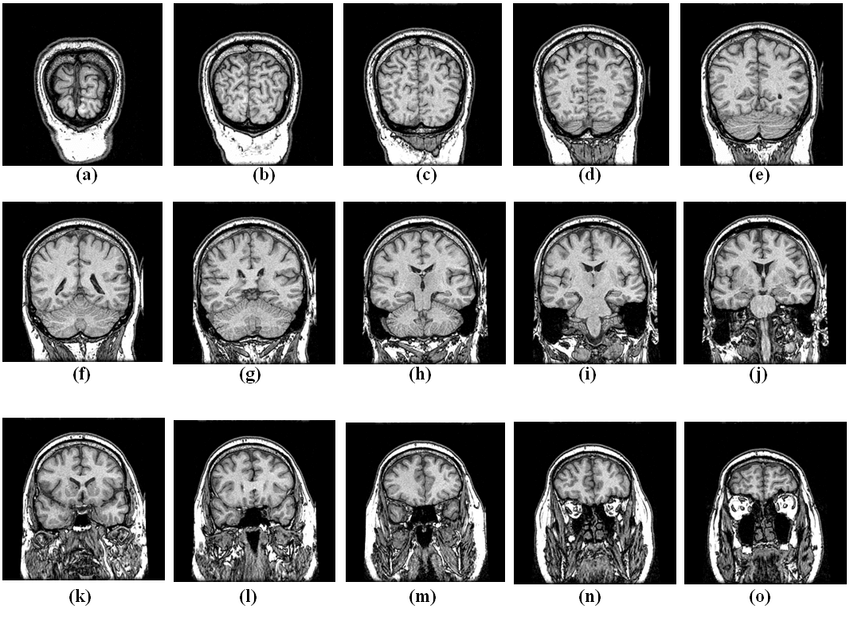
\includegraphics[width=.8\textwidth]{brains.png}
    \end{center}
  \end{figure}
  }
  \only<2>{
    \begin{figure}
      \begin{center}
        \includegraphics[width=.8\textwidth]{weatherstation.png}
      \end{center}
    \end{figure}
  }
\end{frame}

\begin{frame}{Geometry is Hard}
  \begin{itemize}
    \item High-dimensional space is extremely unintuitive
    \item If $V_n(r)$ is the volume of the $n$-dimensional ball with radius $r$, then for any $\varepsilon>0$, $$\lim_{n\to\infty}\frac{V_n(1-\varepsilon)}{V_n(1)}=0$$ i.e., the volume of balls lives almost entirely at the boundary
    \item Trying to analyze many characteristics creates combinatorial problems ($n!$ is big!)
  \end{itemize}
  
\end{frame}

\begin{frame}{Toning It Down}
  \begin{itemize}
    \item Broad idea: high dimensions $\implies$ low dimensions
    \item More specific idea: build a simplicial complex
    \item Simpler idea: build a 1-dimensional simplicial complex (that is, a graph)
    \item Enter: the Mapper algorithm (Singh et al, 2007) \cite{mapper}
    \vspace*{.5cm}
  \begin{figure}
    \begin{center}
      \hspace*{-1cm}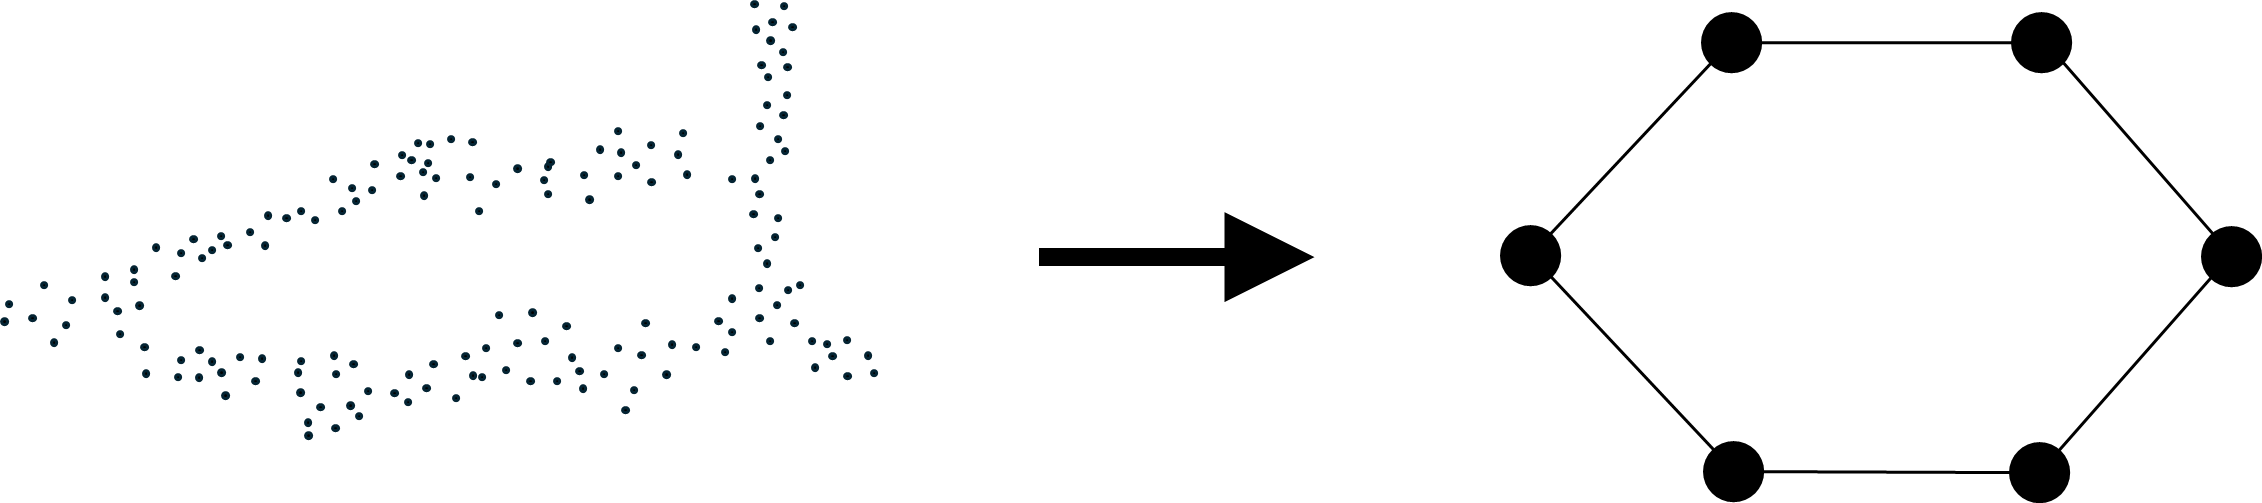
\includegraphics[width=1\textwidth]{datatograph.png}
    \end{center}
  \end{figure}
  \end{itemize}
\end{frame}

\section{Mapper and Its Flavors}
\begin{frame}{Motivation: Reeb Graph}
  \begin{itemize}
    \item Idea: construct graph reflecting level sets of a ``filter'' function
    \item Formally, given a topological space $X$ and a continuous function 
    $f: X\to\mathbb{R}$, define an equivalence relation $\sim$ on $X$ where $x\sim y$ if $x$ and $y$ live in the same connected component of a level set $f^{-1}(c)$ for some $c\in\mathbb{R}$.
    \item The \textbf{Reeb graph}\footnote{Despite names this is not always a graph} is $X/\sim$, taken with the quotient topology.
  \end{itemize}
\end{frame}

\begin{frame}{Motivation: Reeb Graph}
  \begin{figure}
    \begin{center}
      \hspace*{-.6cm}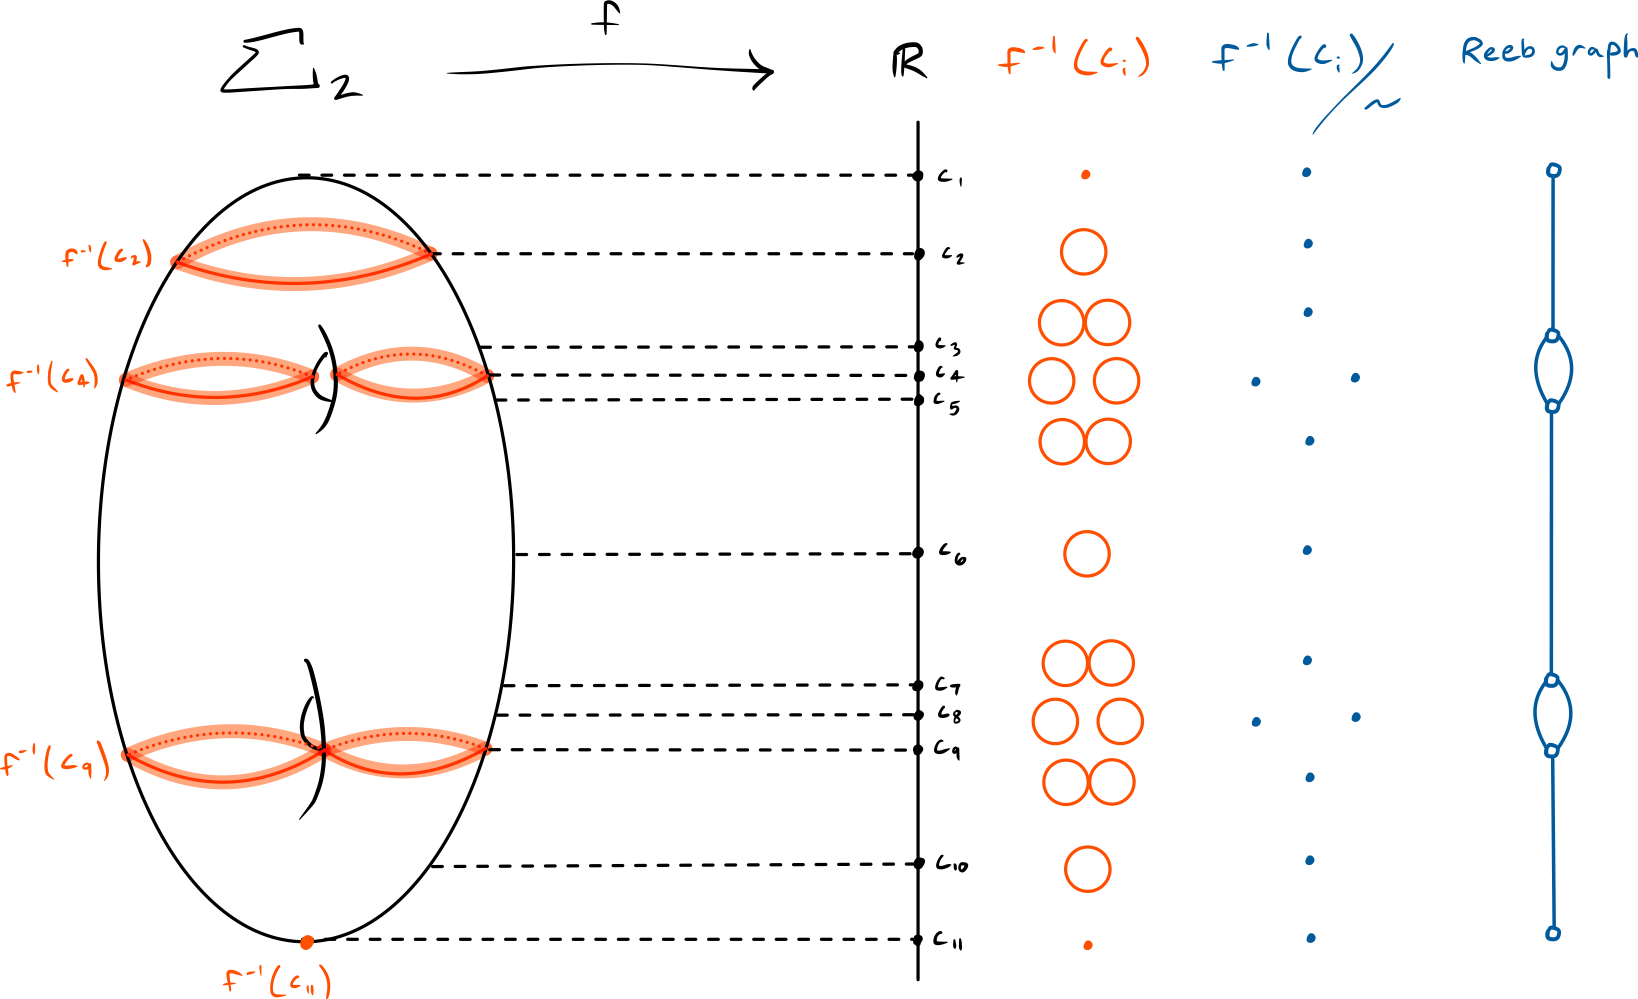
\includegraphics[width=1.1\textwidth]{reeb.png}
    \end{center}
  \end{figure}
\end{frame}

\begin{frame}{Mapper: Original Flavor}
\begin{itemize}
  \item How can we apply this to the discrete setting?
  \item Topological space $X \implies$ point cloud $P$ (a discrete set of points in a space)
  \item Filter function: $f: P\to\mathbb{R}$
  \item Level sets of points $\implies$ level sets of overlapping intervals
  \item Connected components $\implies$ clusters
  \item Quotient space $\implies$ intersection graph
\end{itemize}
\end{frame}

\begin{frame}{Original Mapper Algorithm: Overview}
  \begin{itemize}
    \item Ingredients:
    \begin{itemize}
      \item Point cloud $P$
      \item Filter function $f:P\to\mathbb{R}$
      \item Collection of overlapping intervals $\{I_1, \dots, I_k\}$
      \item Clustering algorithm
    \end{itemize}
    \item Output:
    \begin{itemize}
      \item Finite graph $M$
    \end{itemize}
  \end{itemize}
\end{frame}

\begin{frame}{Point Cloud}
  Our example point cloud will live in $\mathbb{R}^2$:
  \begin{figure}
    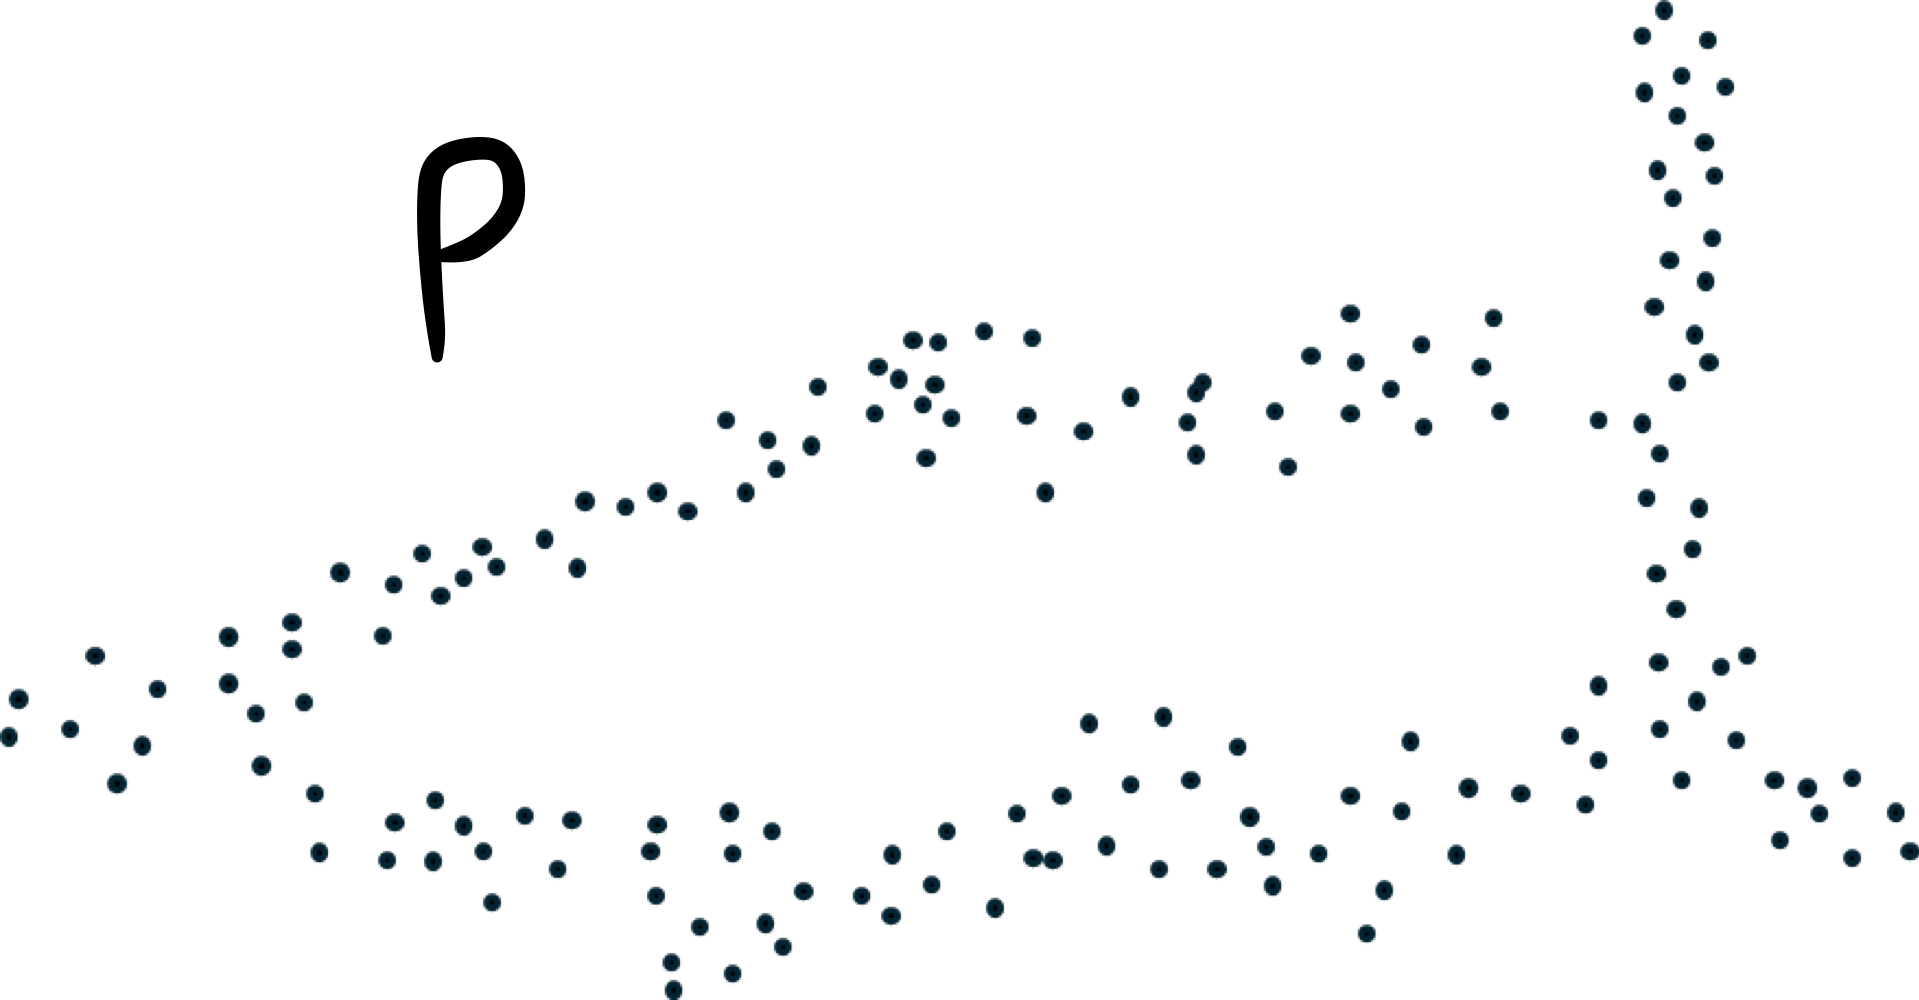
\includegraphics[width=1\textwidth]{pointcloud.png}
  \end{figure}
\end{frame}

\begin{frame}{Filtering}
  \only<1>{\begin{figure}
    \begin{center}
      \vspace*{-4.25cm}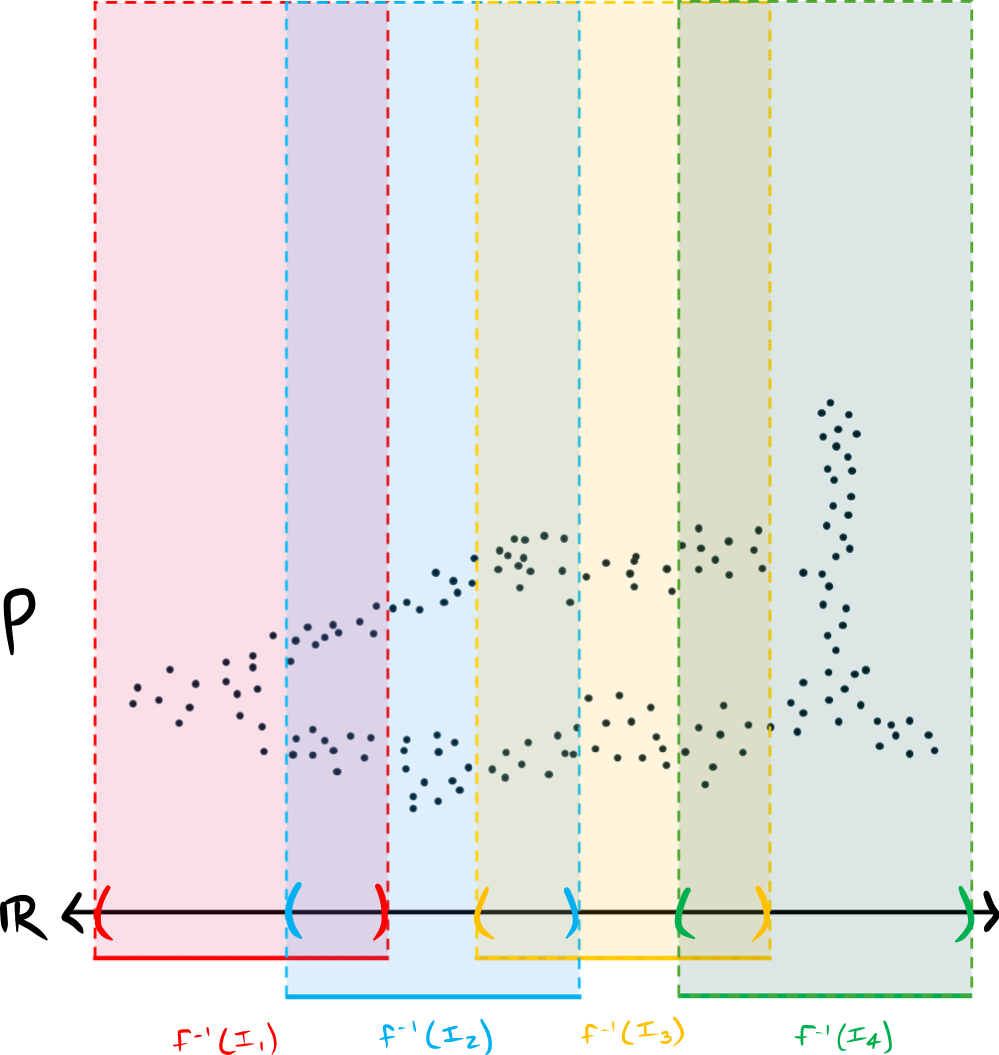
\includegraphics[width=1\textwidth]{filteredposterdata.png}
    \end{center}
  \end{figure}
  Here, $f:P\to\mathbb{R}$ is projection to the $x$-coordinate.}
  \only<2>{\begin{figure}
    \begin{center}
      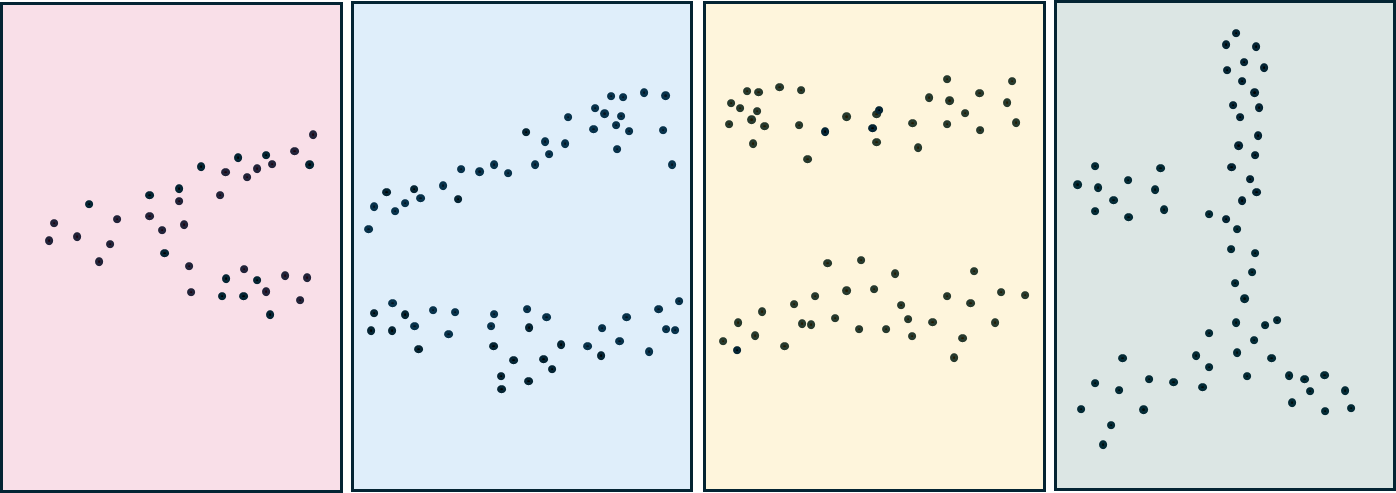
\includegraphics[width=1\textwidth]{bins.png}
    \end{center}
  \end{figure}}
\end{frame}

\begin{frame}{Clustering}
  \begin{figure}
    \begin{center}
      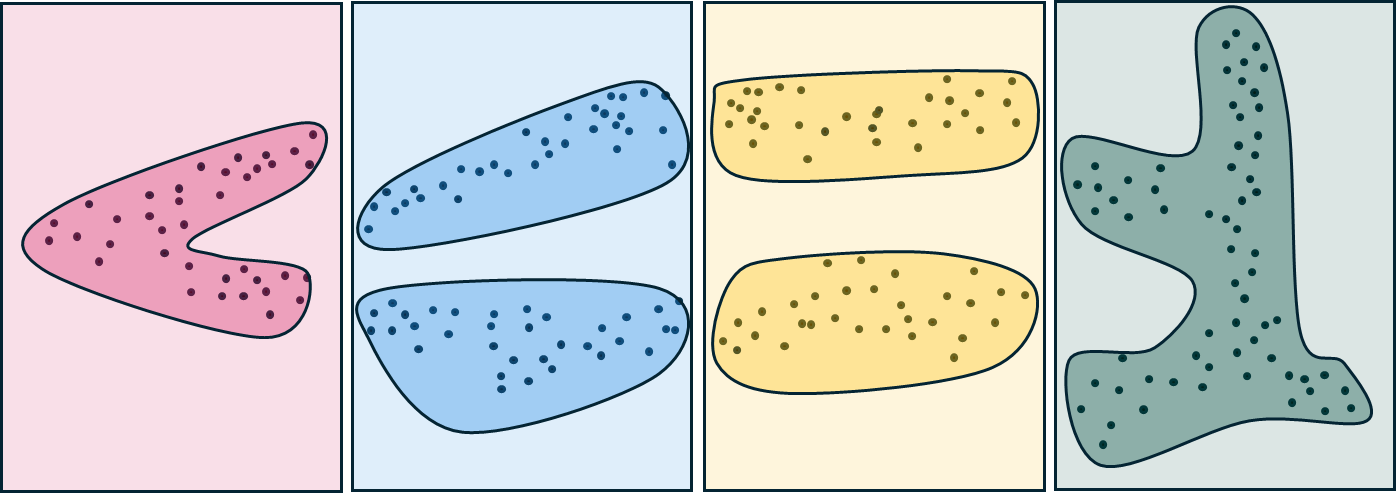
\includegraphics[width=1\textwidth]{posterdataclusters.png}
    \end{center}
  \end{figure}
\end{frame}

\begin{frame}{Overlapping Clusters}
  \begin{figure}
    \begin{center}
      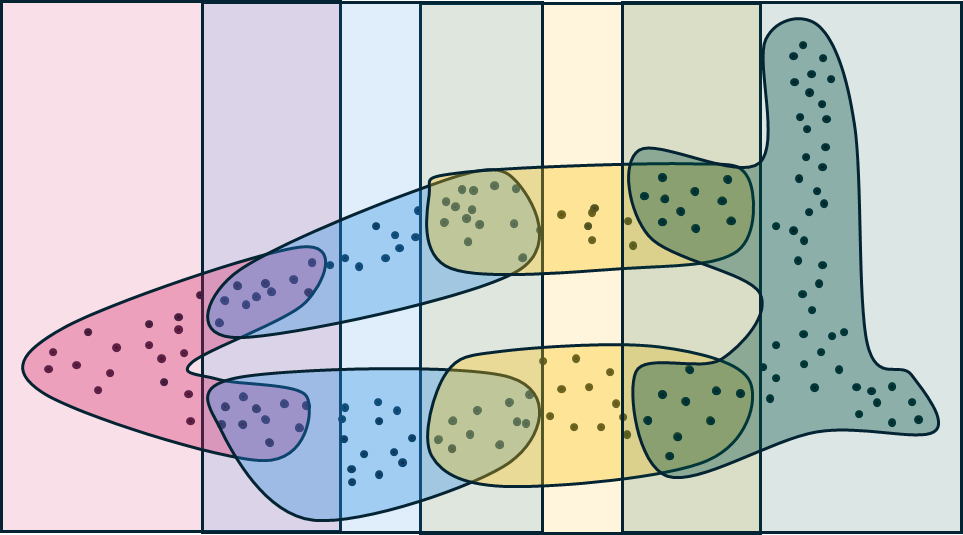
\includegraphics[width=.8\textwidth]{intersectposterdata.png}
    \end{center}
  \end{figure}
\end{frame}

\begin{frame}{Output}
  \begin{figure}
    \begin{center}
      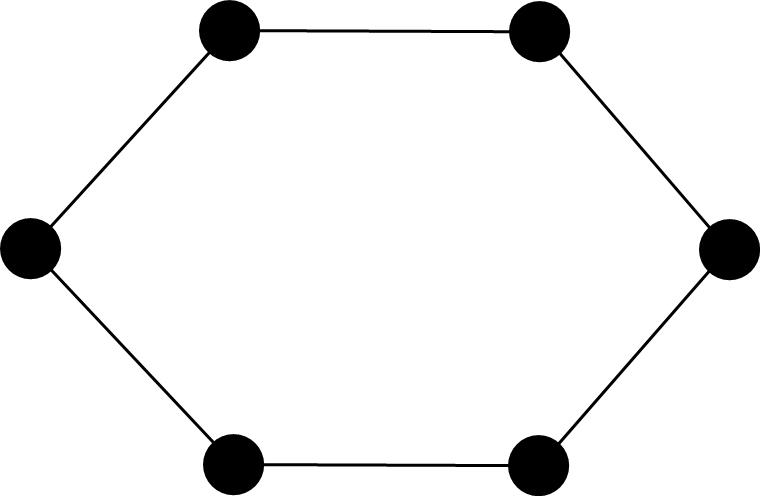
\includegraphics[width=.8\textwidth]{postermapper.png}
    \end{center}
  \end{figure}
\end{frame}

\begin{frame}{Original Mapper: Problems}
  \begin{figure}
    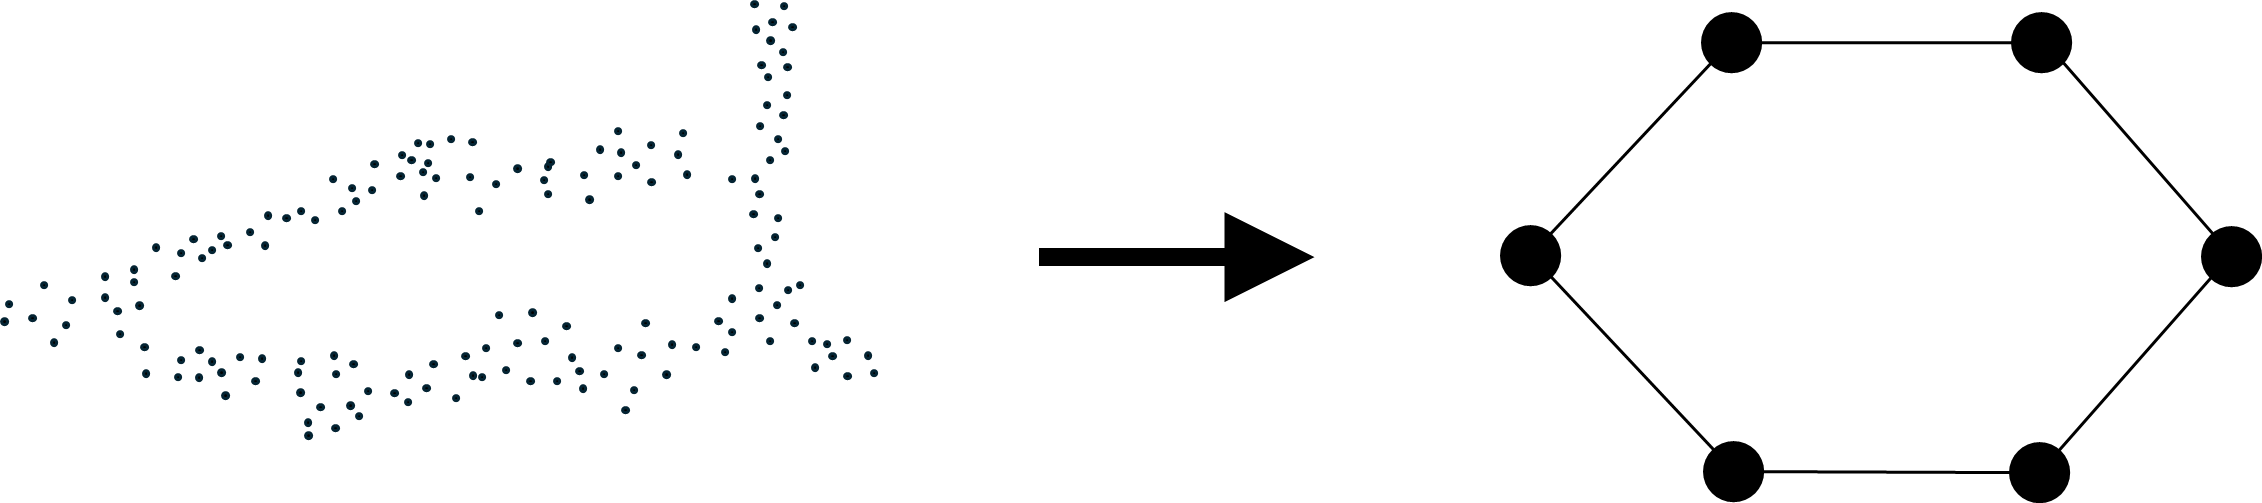
\includegraphics[width=1\textwidth]{datatograph.png}
  \end{figure}
  \begin{itemize}
    \item We lost so much stuff! Clustering takes work.
    \item Graphs are abstract combinatorial structures; they convey no other information
    \item Potentially interesting features can ``bypass'' the filter
    \item Large number of parameters complicates effectiveness
    \item Output heavily depends on choice of clustering method
  \end{itemize}
\end{frame}

\begin{frame}{Speaking of Clustering Methods...}
  \begin{figure}
    \begin{center}
      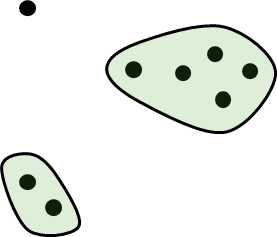
\includegraphics[width=.5\textwidth]{threeclusters.png}
    \end{center}
  \end{figure}
  There are a large variety of clustering algorithms, including:
  \begin{itemize}
      \item Hierarchical clustering
      \item $k$-means clustering (centroid based)
      \item DBSCAN (density based)
      \item Topological clustering
  \end{itemize}
\end{frame}

\begin{frame}{How to Cluster, Hierarchically}
  \begin{itemize}
    \item Two ingredients:
    \begin{itemize}
      \item A discrete set of points $X$, equipped with a distance function $d:X\times X\to\mathbb{R}$
      \item A \textbf{linking criterion}, a (partial) function $\ell: \mathscr{P}(X)\times\mathscr{P}(X)\to\mathbb{R}$ which measures the distance between disjoint sets of points
    \end{itemize}
    \item Process:
    \begin{enumerate}
      \item Begin by considering each point as an individual cluster as part of a collection $\mathcal{C}$.
      \item Find the two $A,B\in\mathcal{C}$ that minimize $\ell$. Merge these clusters.
      \item Repeat step 2 until $\mathcal{C}$ consists of up to a single cluster.
    \end{enumerate}
    \item We record the resulting hierarchy of clusters using a \textbf{dendrogram}, which records information about the merging process.
  \end{itemize}
\end{frame}

\begin{frame}{Example: Single Linkage Clustering}
  \begin{itemize}
    \item Data: 8 points in $\mathbb{R}^2$, with the usual metric
    \vspace*{.5cm}
    \begin{figure}
      \begin{center}
        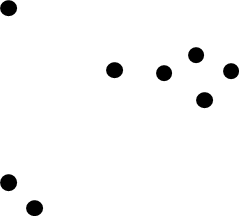
\includegraphics[width=.35\textwidth]{cluster0.png}
      \end{center}
    \end{figure}
    \vspace*{.5cm}
    \item Linking criterion: $$\ell(A, B) = \min_{a\in A, b\in B}\{d(a,b)\}$$
    \item Starting dendrogram:
    \begin{figure}
      \begin{center}
        
\includegraphics[width=.4\textwidth]{eightdend.png}
      \end{center}
    \end{figure}
  \end{itemize}
\end{frame}

\begin{frame}{Single Linkage Clustering In Action}
  $$\ell(A, B) = \min_{a\in A, b\in B}\{d(a,b)\}$$
  \only<1>{\begin{figure}\begin{center}
    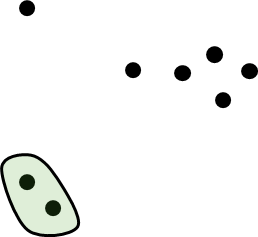
\includegraphics[width=.35\textwidth]{sevenclusters.png}
  \end{center}\end{figure}
  We merge edges at a height proportional to the corresponding value of $\ell$ (the merge height):
  \begin{figure}
    \begin{center}
      
\includegraphics[width=.4\textwidth]{sevendend.png}
    \end{center}
  \end{figure}
  }
 \only<2>{\begin{figure}[!h]
    \centering
    \begin{subfigure}{.2\linewidth}
      \centering
      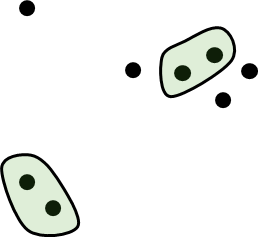
\includegraphics[width=1.75\textwidth]{sixclusters.png}
    \end{subfigure}%
    \hspace{5em}
    \begin{subfigure}{.5\linewidth}
      \centering
      
\includegraphics[width=.9\textwidth]{sixdend.png}
    \end{subfigure}
    \end{figure}}

    \only<3>{\begin{figure}[!h]
      \centering
      \begin{subfigure}{.2\linewidth}
        \centering
        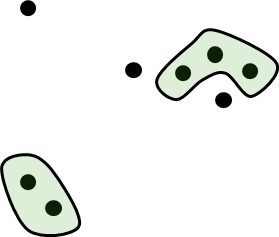
\includegraphics[width=1.75\textwidth]{fiveclusters.png}
      \end{subfigure}%
      \hspace{5em}
      \begin{subfigure}{.5\linewidth}
        \centering
        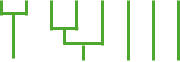
\includegraphics[width=.9\textwidth]{fivedend.png}
      \end{subfigure}
      \end{figure}}

      \only<4>{\begin{figure}[!h]
        \centering
        \begin{subfigure}{.2\linewidth}
          \centering
          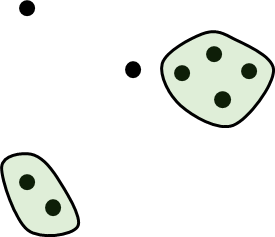
\includegraphics[width=1.75\textwidth]{fourclusters.png}
        \end{subfigure}%
        \hspace{5em}
        \begin{subfigure}{.5\linewidth}
          \centering
          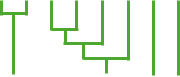
\includegraphics[width=.9\textwidth]{fourdend.png}
        \end{subfigure}
        \end{figure}}

 \only<5>{\begin{figure}[!h]
    \centering
    \begin{subfigure}{.2\linewidth}
      \centering
      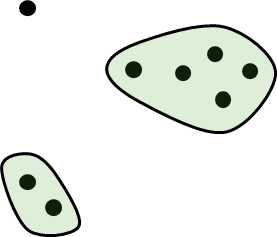
\includegraphics[width=1.75\textwidth]{threeclusters.png}
    \end{subfigure}%
    \hspace{5em}
    \begin{subfigure}{.5\linewidth}
      \centering
      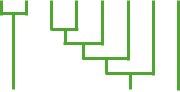
\includegraphics[width=.9\textwidth]{threedend.png}
    \end{subfigure}
    \end{figure}}

 \only<6>{\begin{figure}[!h]
    \centering
    \begin{subfigure}{.25\linewidth}
      \centering
      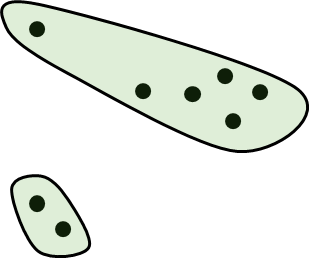
\includegraphics[width=1.75\textwidth]{twoclusters.png}
    \end{subfigure}%
    \hspace{5em}
    \begin{subfigure}{.5\linewidth}
      \centering
      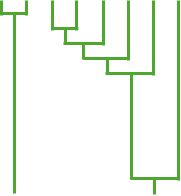
\includegraphics[width=.8\textwidth]{twodend.png}
    \end{subfigure}
    \end{figure}}

    \only<7>{\begin{figure}[!h]
      \centering
      \begin{subfigure}{.25\linewidth}
        \centering
        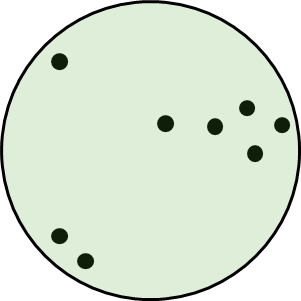
\includegraphics[width=1.75\textwidth]{onecluster.png}
      \end{subfigure}%
      \hspace{5em}
      \begin{subfigure}{.4\linewidth}
        \centering
        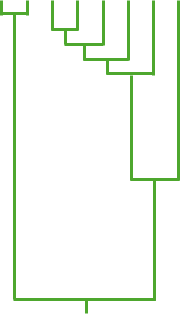
\includegraphics[width=.75\textwidth]{onedend.png}
      \end{subfigure}
      \end{figure}}
\end{frame}

\begin{frame}{Ballmapper (Dłotko, 2019)}
  \begin{itemize}
    \item Original flavor has a lot of choices to make
    \item Idea: come up with a one (ish)-parameter Mapper
    \item \textbf{Ballmapper} \cite{ballmapper}: in place of a conventional filter, cover the dataset with overlapping $\varepsilon$-balls
    \item Specifically, we want a cover $C = \bigcup_i B(x_i, \varepsilon)$ such that:
    \begin{itemize}
      \item Every datapoint $x$ is contained in $B(x_i, \varepsilon)$ for some $x_i$
      \item If $x_j$ is a ball center, then the only ball containing it is $B(x_j, \varepsilon)$
    \end{itemize}
    \item Graph construction unchanged
  \end{itemize}
  
\end{frame}

\begin{frame}{Ballmapper Algorithm: Overview}
  \begin{itemize}
    \item Ingredients:
    \begin{itemize}
      \item Point cloud $P$ with distance function $d$
      \item Ball radius $\varepsilon > 0$
      \item Suitable cover of data $\bigcup B_\varepsilon(x_i)$
    \end{itemize}
    \item Output:
    \begin{itemize}
      \item Finite graph $BM$
    \end{itemize}
  \end{itemize}
\end{frame}

\begin{frame}{Balling the Data}
  \begin{itemize}
    \item Can be done quickly with a greedy method
    \item May also use $k$-means clustering, etc.
  \end{itemize}
  \begin{figure}
    \begin{center}
      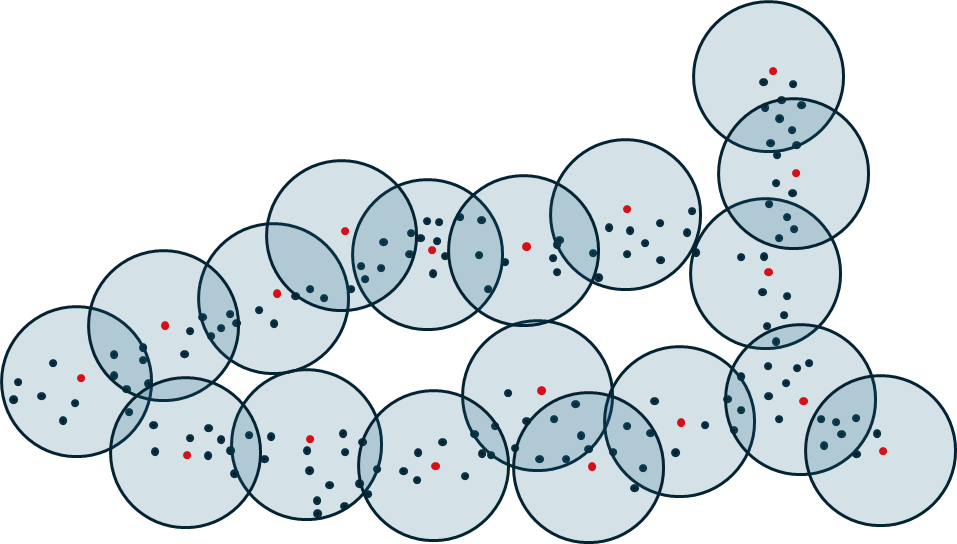
\includegraphics[width=1\textwidth]{ballcover.png}
    \end{center}
  \end{figure}

\end{frame}

\begin{frame}{Output}
  \begin{figure}
    \begin{center}
      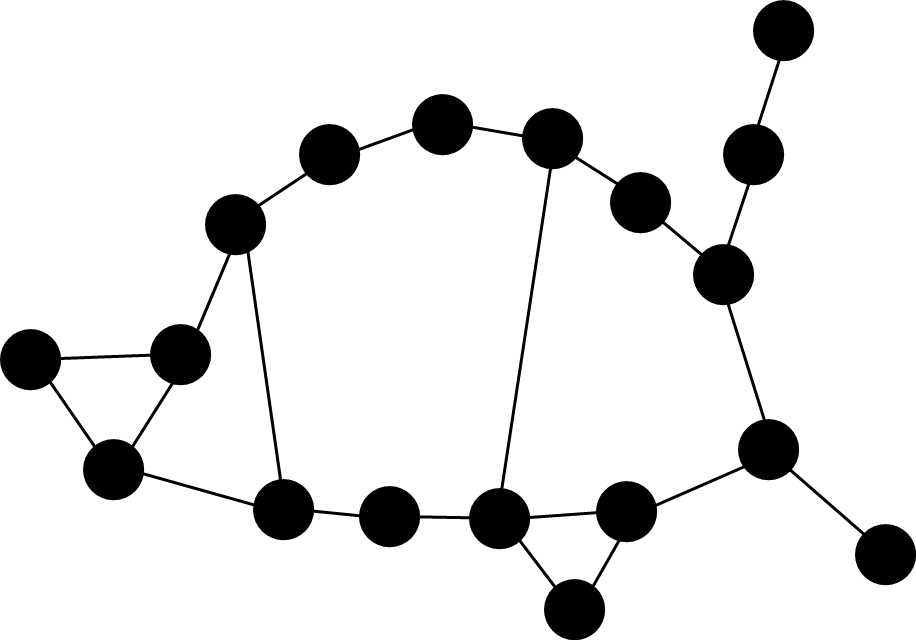
\includegraphics[width=1\textwidth]{ballmapperposter.png}
    \end{center}
  \end{figure}
\end{frame}

\begin{frame}{Ballmapper: Problems}
  \begin{figure}
    \begin{center}
      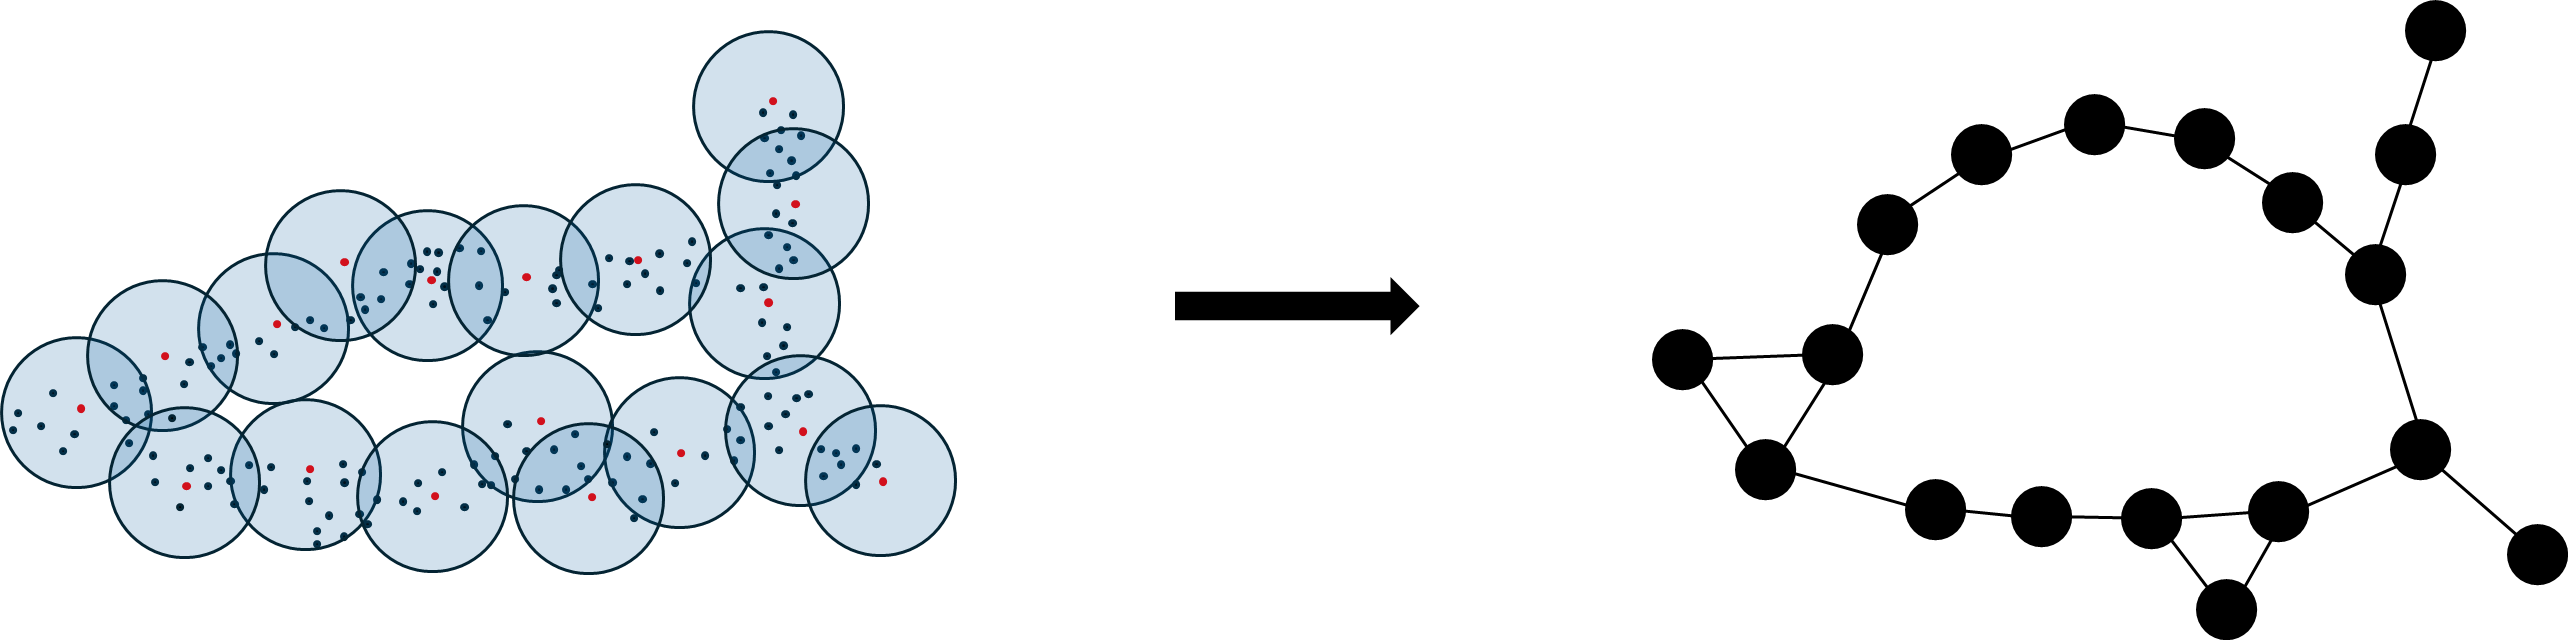
\includegraphics[width=1\textwidth]{ballmapperarrow.png}
    \end{center}
    \begin{itemize}
      \item Output is still just a graph!
      \item Balls become black boxes
      \item Can be quite noisy if $\varepsilon$ is too small, and meaningless for $\varepsilon$ too large
    \end{itemize}
  \end{figure}
\end{frame}

\begin{frame}{Refined Ballmapper}
  \begin{itemize}
    \item Idea: combine Ball filtering and Original clustering
    \item Bin by balling, then cluster within balls as in Original
    \item Allows for comparison of two different metrics\footnote{Could be not strictly metrics!} at the same time on the same data
  \end{itemize}
  
\end{frame}

\begin{frame}{Refined Ballmapper: Overview}
  \begin{itemize}
    \item Ingredients:
    \begin{itemize}
      \item Point cloud $P$ with distance function $d$
      \item Ball radius $\varepsilon > 0$
      \item Suitable cover of data $\bigcup B_\varepsilon(x_i)$
      \item Clustering algorithm
    \end{itemize}
    \item Output:
    \begin{itemize}
      \item Finite graph $RBM$
    \end{itemize}
  \end{itemize}
\end{frame}

\begin{frame}{Standard Ballmapper}
  \begin{figure}
    \begin{center}
      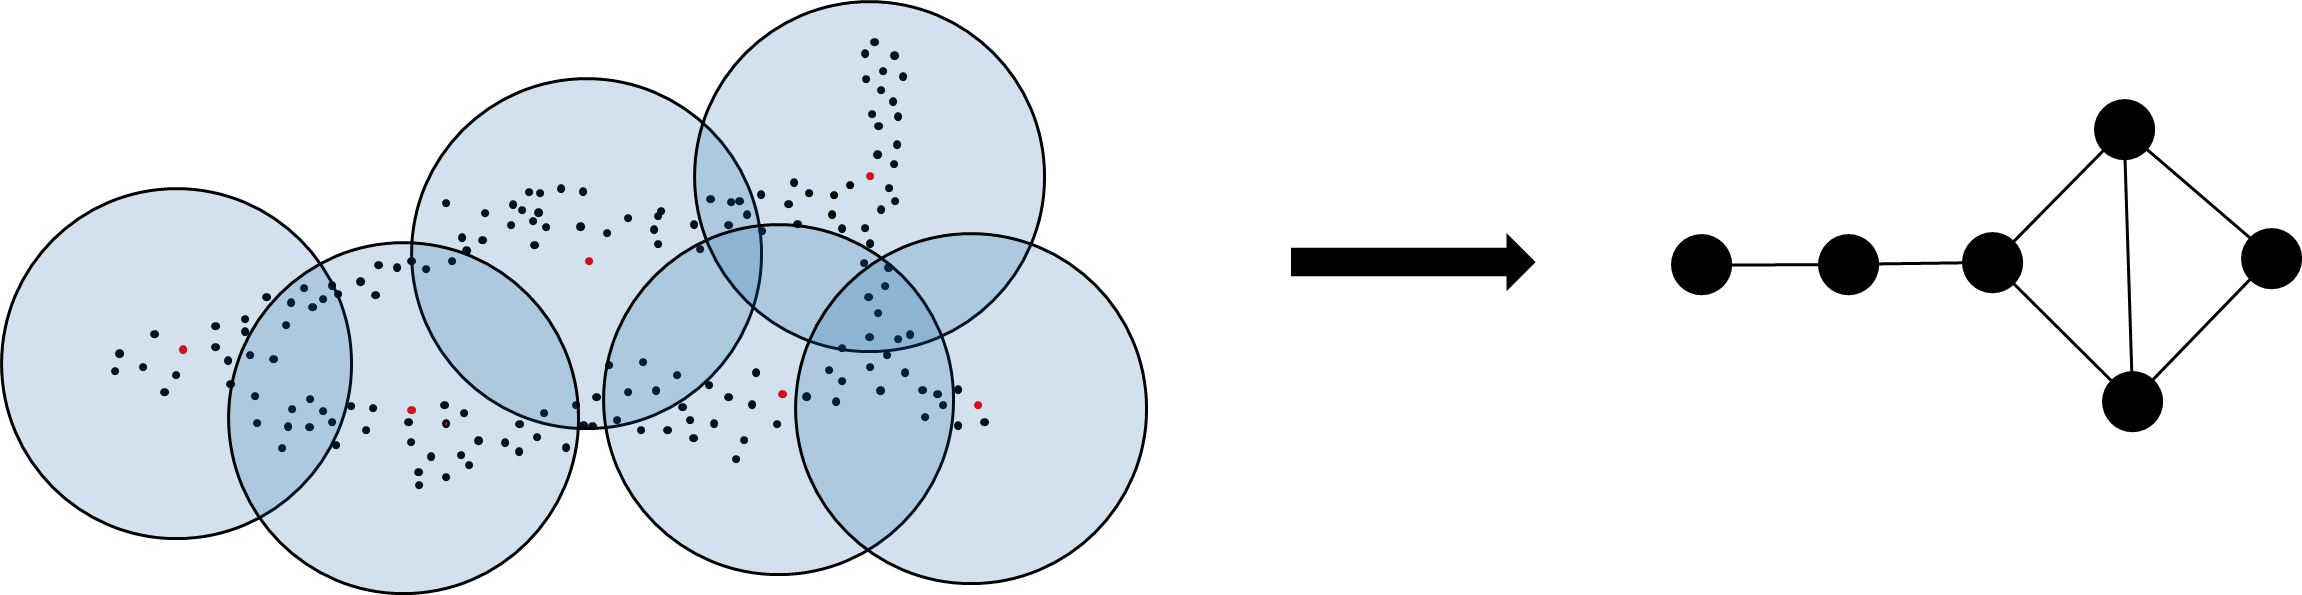
\includegraphics[width=1\textwidth]{prerefined.png}
    \end{center}
  \end{figure}
\end{frame}

\begin{frame}{Balls as Bins}
  \begin{figure}
    \begin{center}
      \hspace*{-.5cm}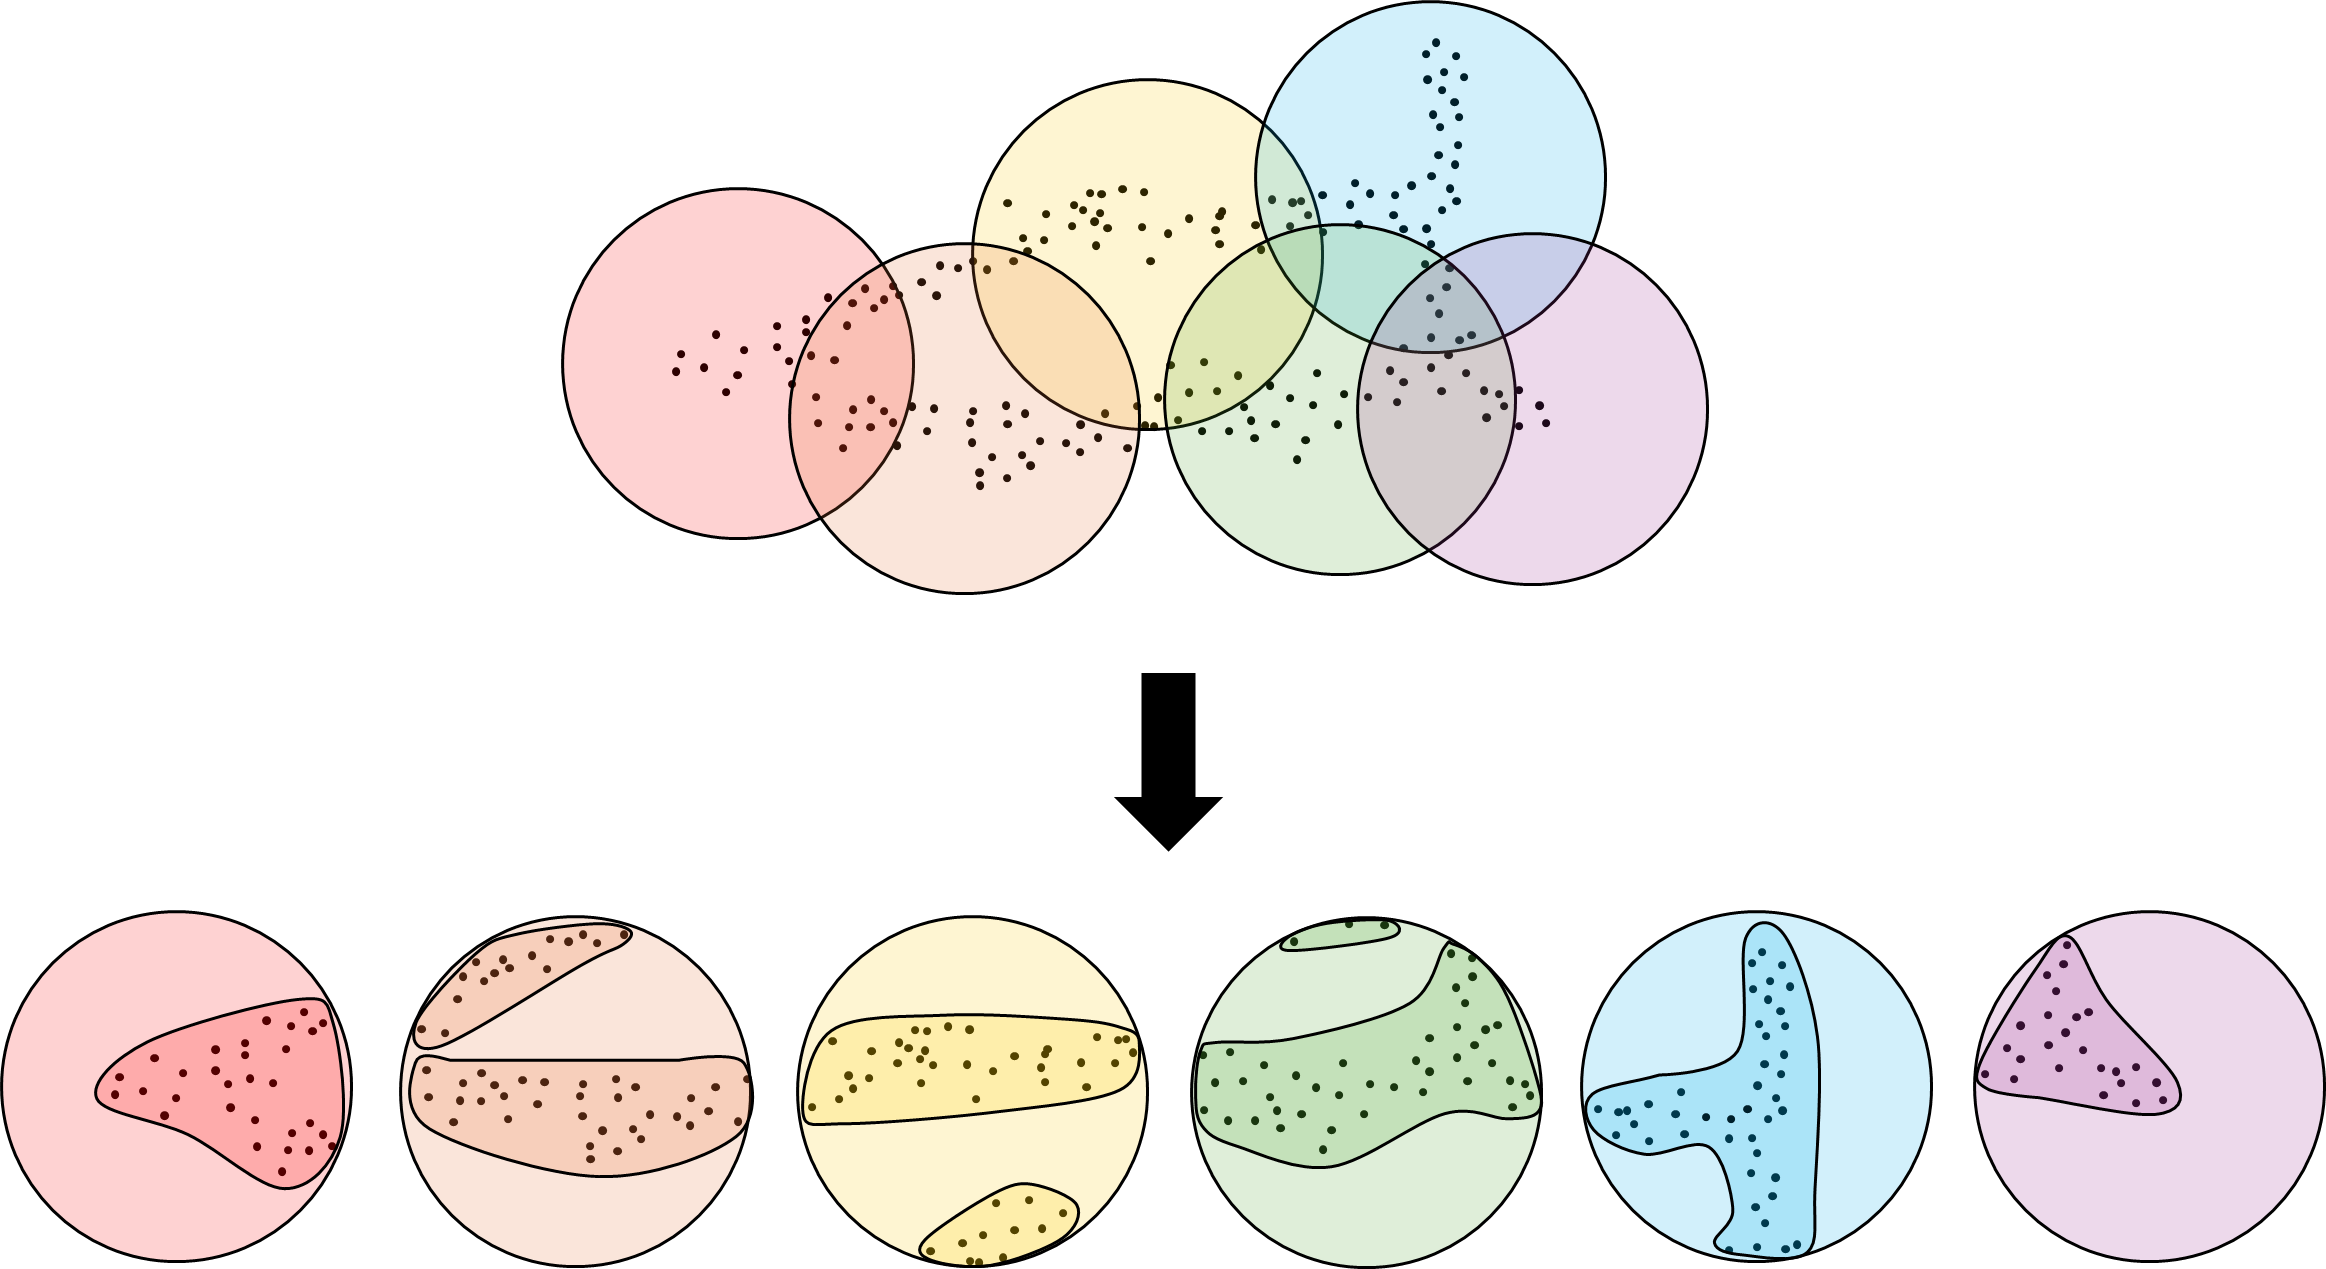
\includegraphics[width=1.1\textwidth]{ballclustering.png}
    \end{center}
  \end{figure}
\end{frame}

\begin{frame}{Balls Together}
  \begin{figure}
    \begin{center}
      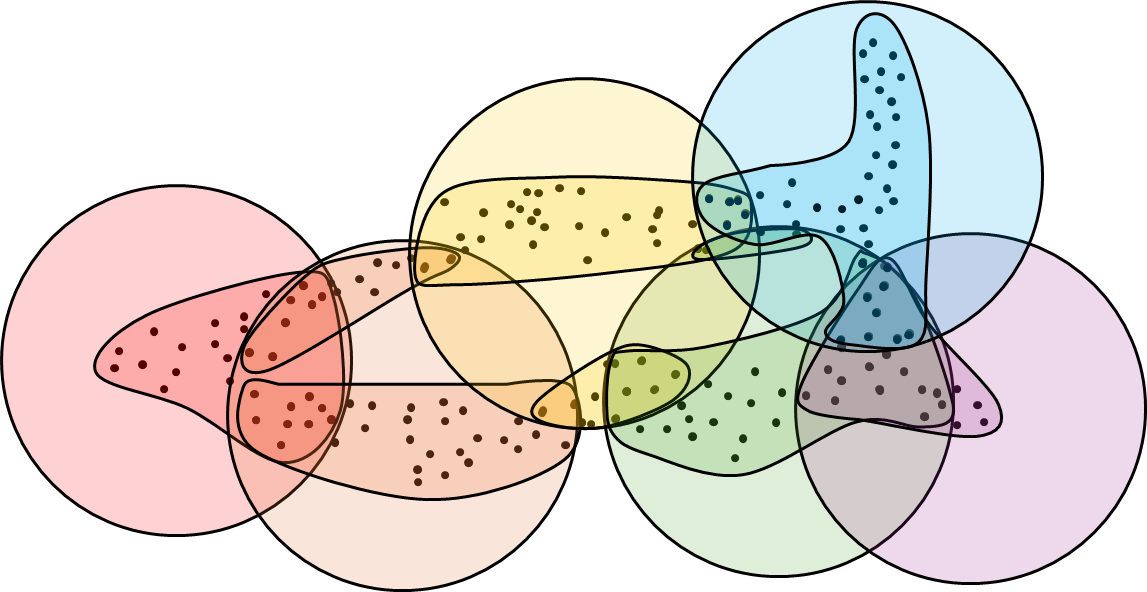
\includegraphics[width=1\textwidth]{intersectingballs.png}
    \end{center}
  \end{figure}
\end{frame}

\begin{frame}{Output}
\begin{figure}
  \begin{center}
    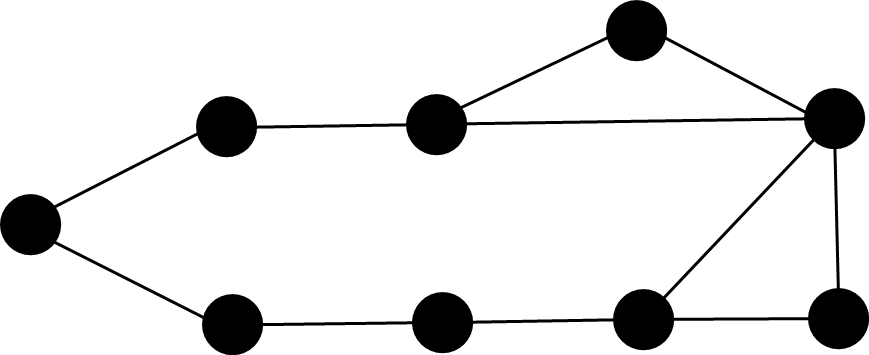
\includegraphics[width=1\textwidth]{rballmapper.png}
  \end{center}
\end{figure}
\end{frame}
  
\begin{frame}{Refined Ballmapper: Problems}
  \begin{figure}
    \begin{center}
      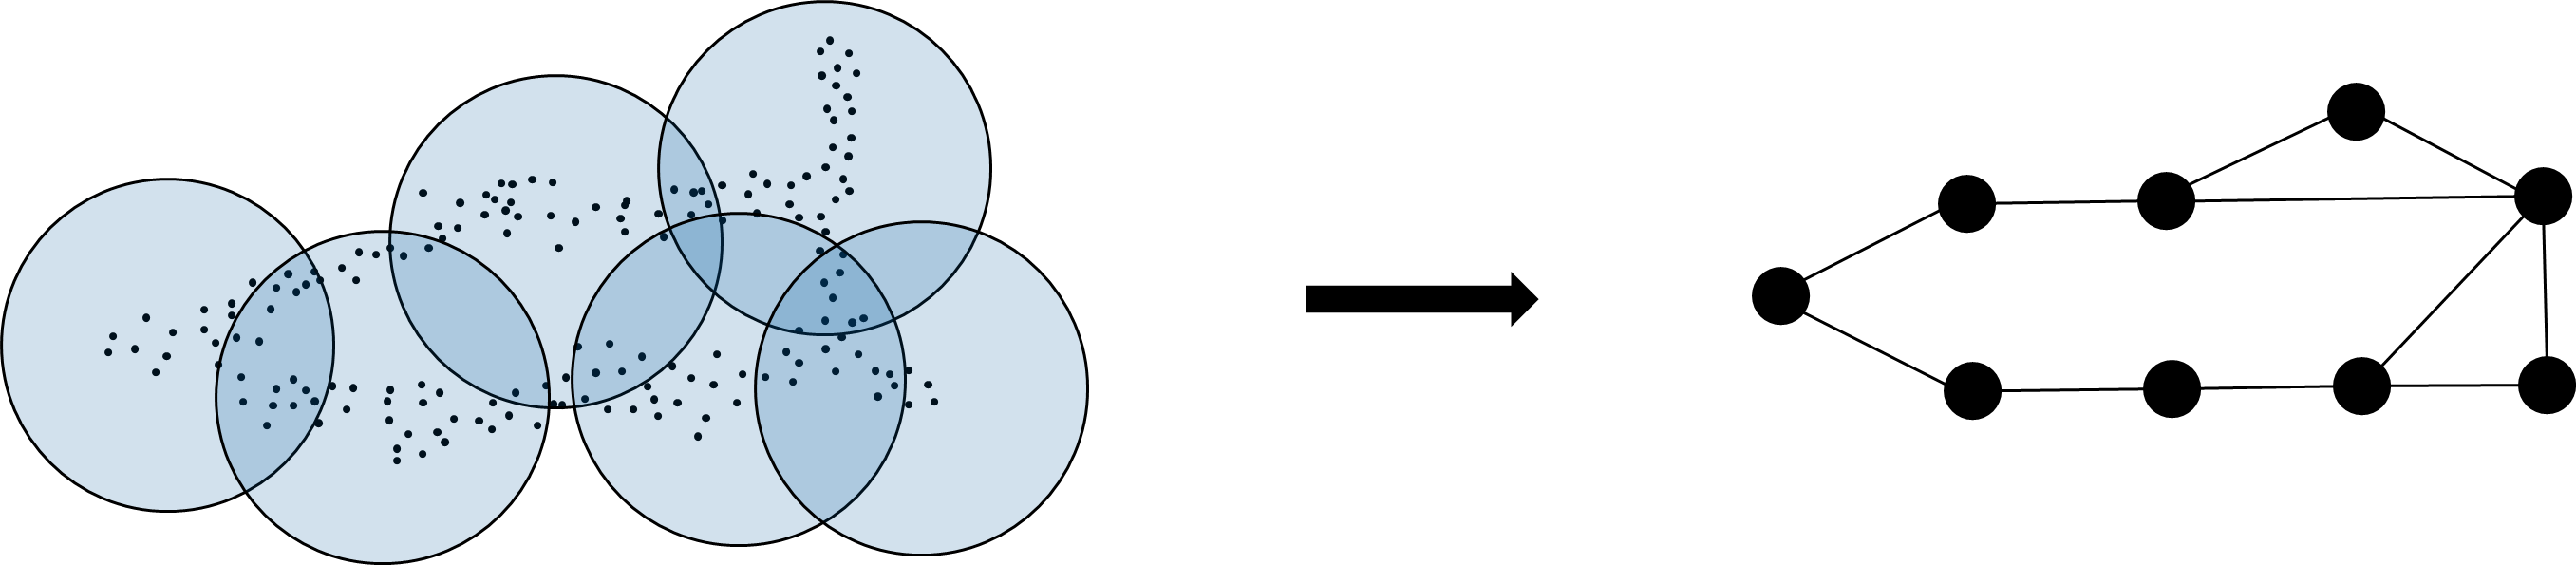
\includegraphics[width=1\textwidth]{rbmarrow.png}
    \end{center}
  \end{figure}
  \begin{itemize}
    \item Choice of cover now strongly influences meaningfulness of clusters
    \item Choice of clustering algorithm is still an issue
    \item Still have that graph problem!
  \end{itemize}
\end{frame}

\section{Cytoscape to the Rescue}
\begin{frame}{What is Cytoscape?}
  \begin{itemize}
    \item Powerful network analysis software (written in Java)
    \item Used primarily by bioinformaticists but is a general use program
  \end{itemize}
  \begin{figure}
    \begin{center}
      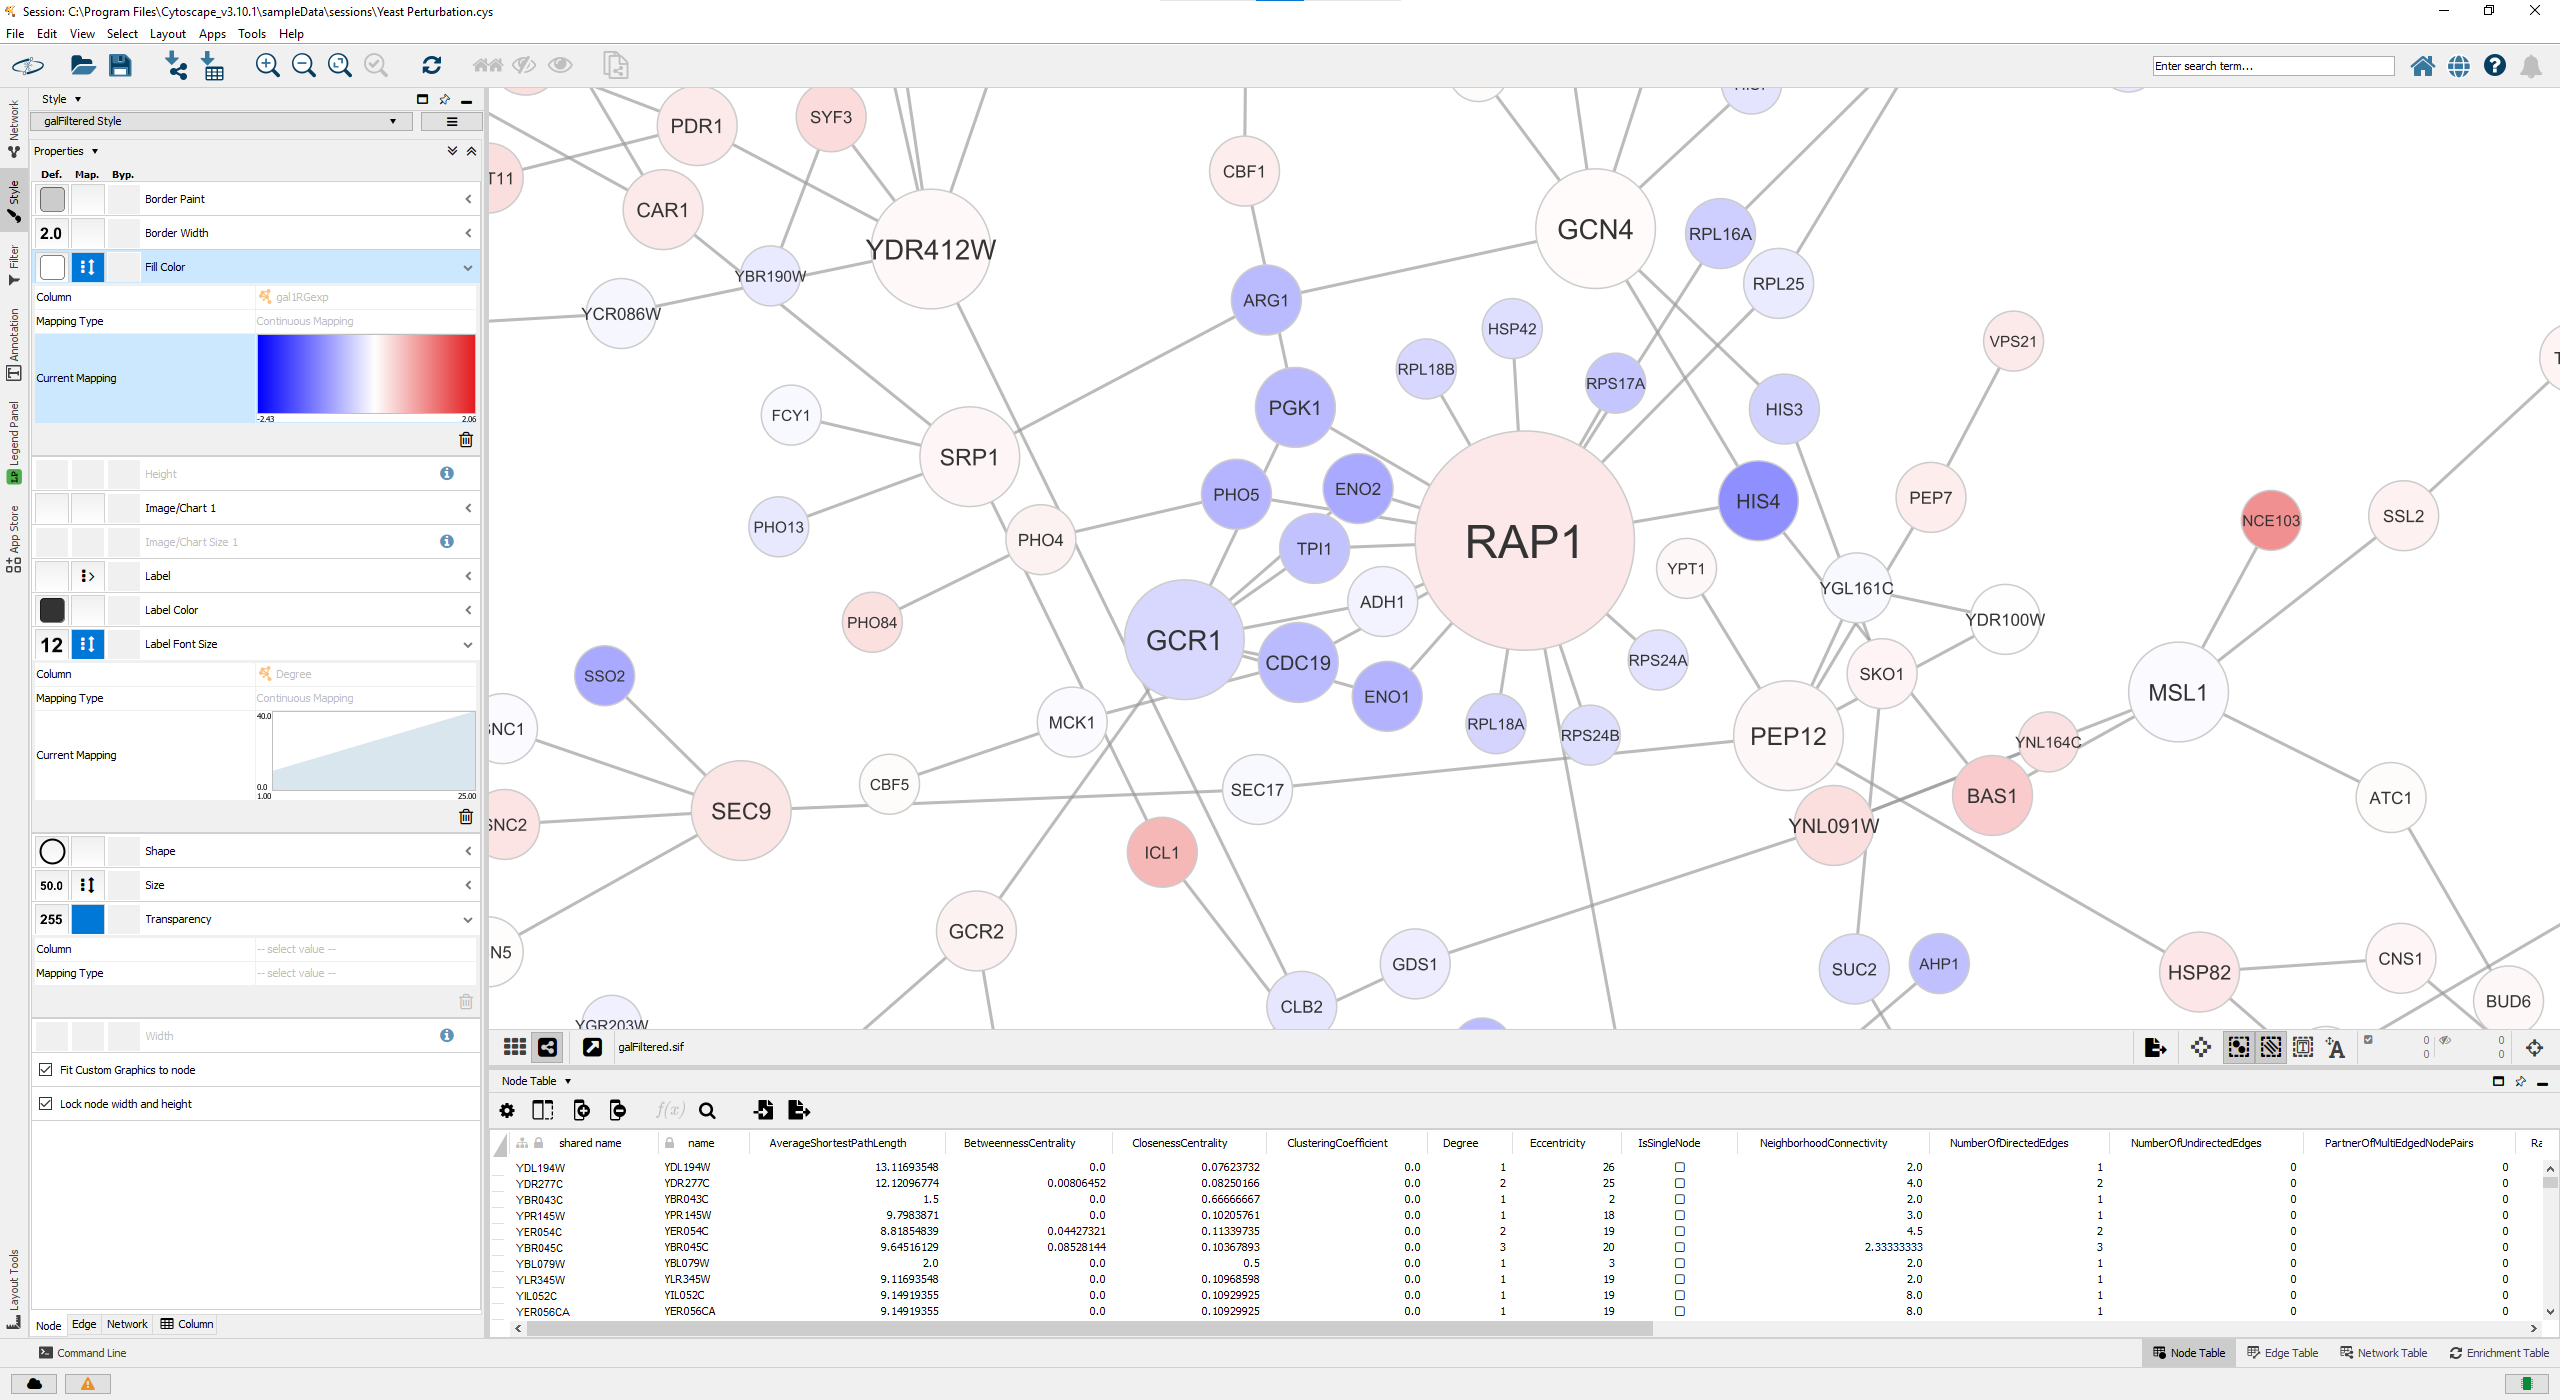
\includegraphics[width=1\textwidth]{cytoyeast.png}
    \end{center}
  \end{figure}
\end{frame}

\begin{frame}{Features}
  \begin{itemize}
    \item Networks are stored as separate tables of nodes and edges
    \item Tables can be augmented with any number or type of columns
    \item Any column can then be associated with a visual characteristic of the network
  \end{itemize}
  \begin{figure}
    \begin{center}
      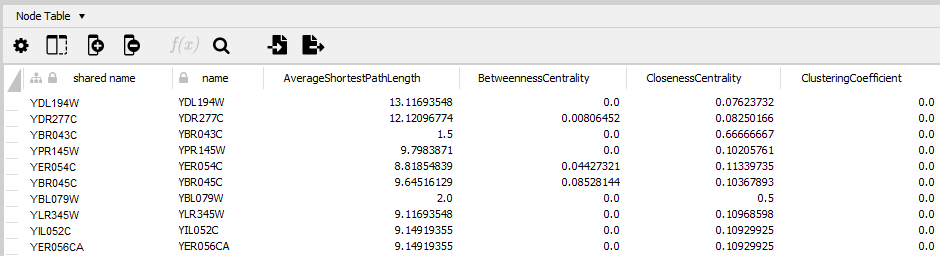
\includegraphics[width=1\textwidth]{nodetable.png}
    \end{center}
  \end{figure}
\end{frame}

\begin{frame}{Styling Mapper: Vertices}
  \begin{itemize}
    \item Node size/label $\to$ cluster size
    \item Node border color $\to$ associated level set/filter value/ball
    \item Node fill color $\to$ cluster dispersion
  \end{itemize}
  \begin{figure}
    \begin{center}
      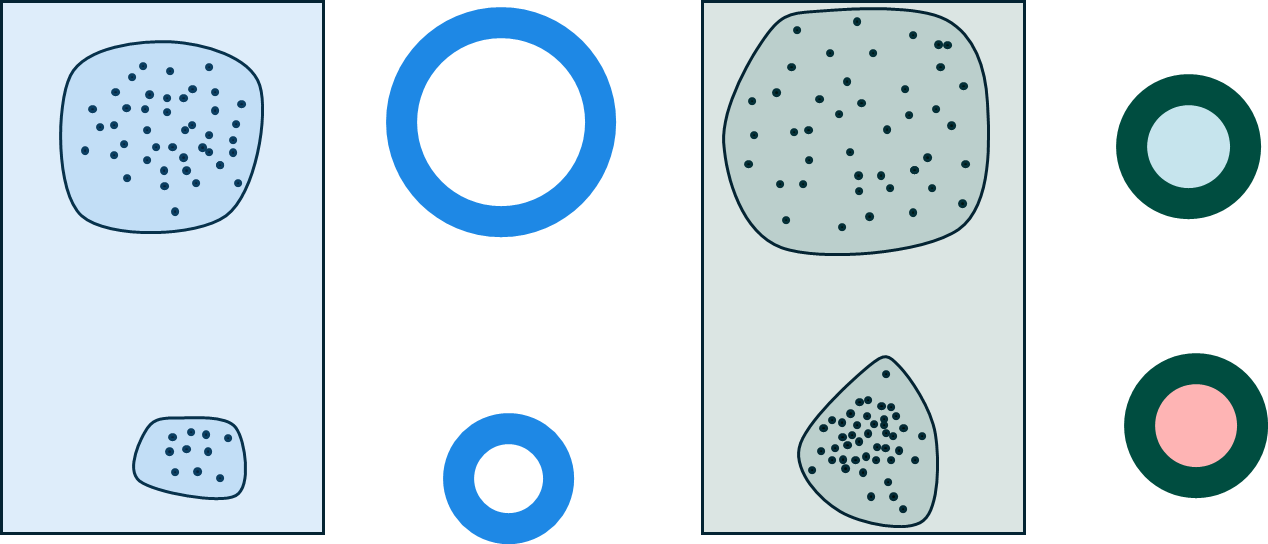
\includegraphics[width=1\textwidth]{nodestyling.png}
    \end{center}
  \end{figure}
\end{frame}

\begin{frame}{Styling Mapper: Edges}
  \begin{itemize}
    \item Edge thickness/opacity $\to$ cluster intersection strength
    \item Edge label $\to$ cluster intersection size
  \end{itemize}
  \begin{figure}
    \begin{center}
      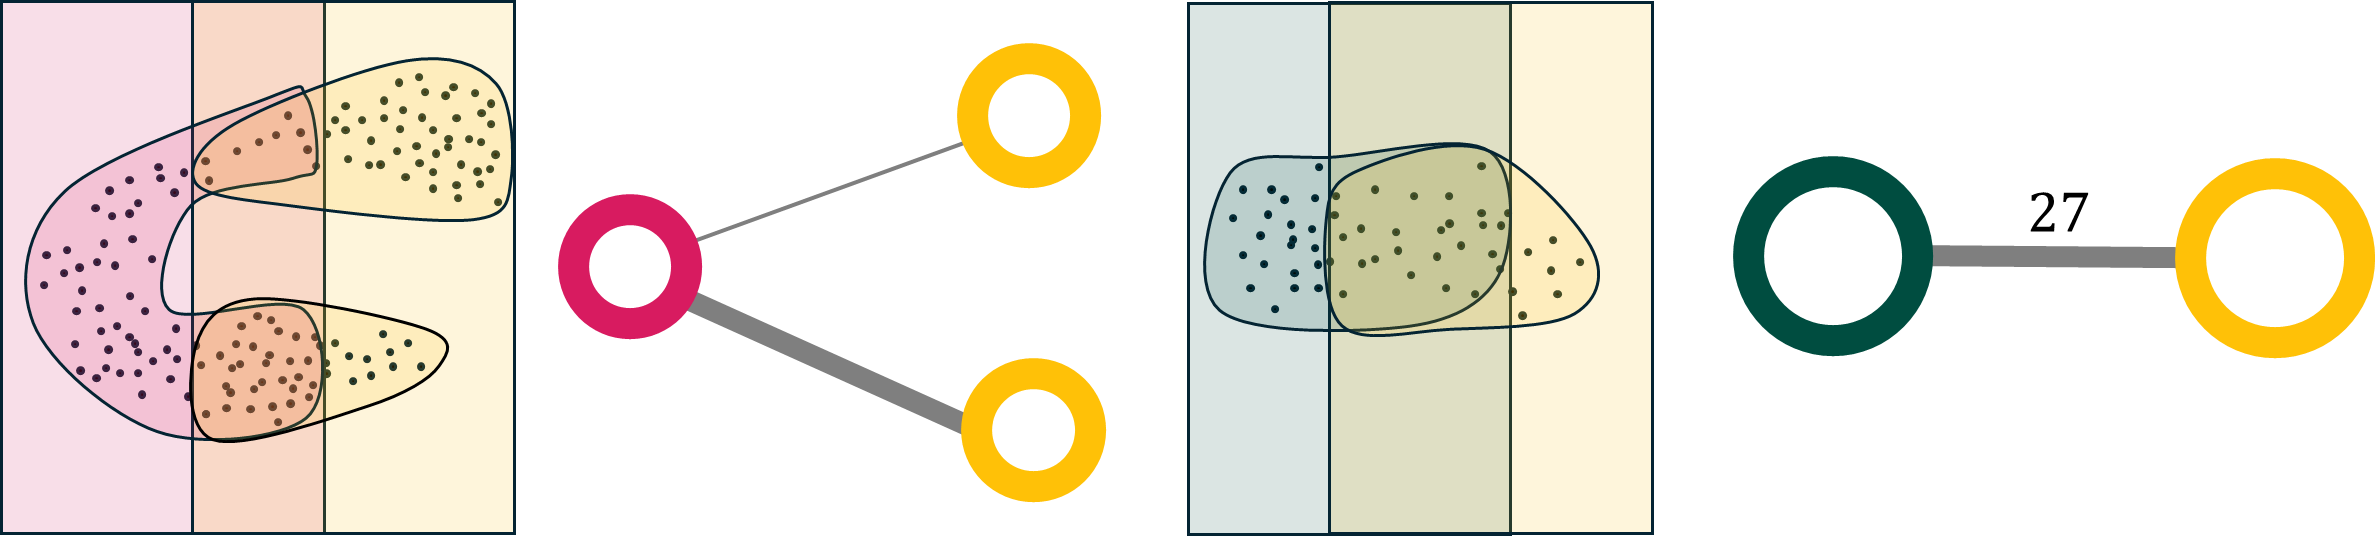
\includegraphics[width=1.05\textwidth]{edgestyling.png}
    \end{center}
  \end{figure}
\end{frame}

\begin{frame}{Exploring the Graph}
  \begin{itemize}
    \item Cytoscape can calculate classical network statistics
    \begin{itemize}
      \item Centrality measures
      \item Clustering coefficients
      \item Modularity classes
    \end{itemize}
    \item We can filter out nodes/edges by characteristics
  \end{itemize}
  \begin{figure}
    \begin{center}
      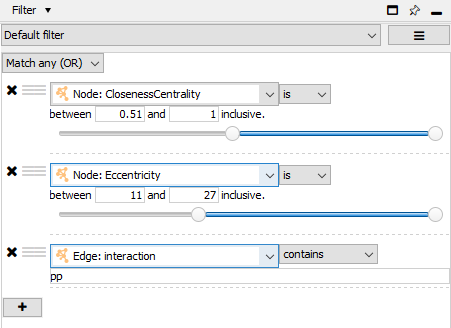
\includegraphics[width=.65\textwidth]{cytofilter.png}
    \end{center}
  \end{figure}
\end{frame}

\begin{frame}{Possible Capabilities}
  \begin{itemize}
    \item Cytoscape is open source and was designed to be modified
    \item Possible projects here include:
    \begin{itemize}
      \item Assign energy function to edges and apply layout algorithm
      \item Animation between networks (say, from RBM to BM or reverse)
      \item More graph algorithms (finding cores, clique detection, etc)
    \end{itemize}
  \end{itemize}
  
\end{frame}
\section{Aptamers}
\begin{frame}{Biology CliffNotes CliffNotes}
  \begin{itemize}
    \item RNA (ribonucleic acid) and DNA (deoxyribonucleic acid) are polymers which carry genetic sequences and have additional structure
  \end{itemize}
  \begin{figure}
    \begin{center}
      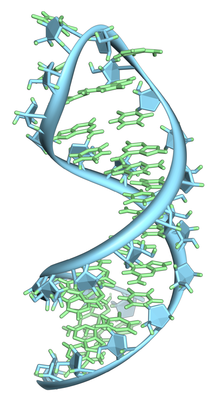
\includegraphics[width=.3\textwidth]{rna.png}
    \end{center}
  \end{figure}
\end{frame}

\begin{frame}{RNA and DNA}
  \begin{figure}
    \begin{center}
      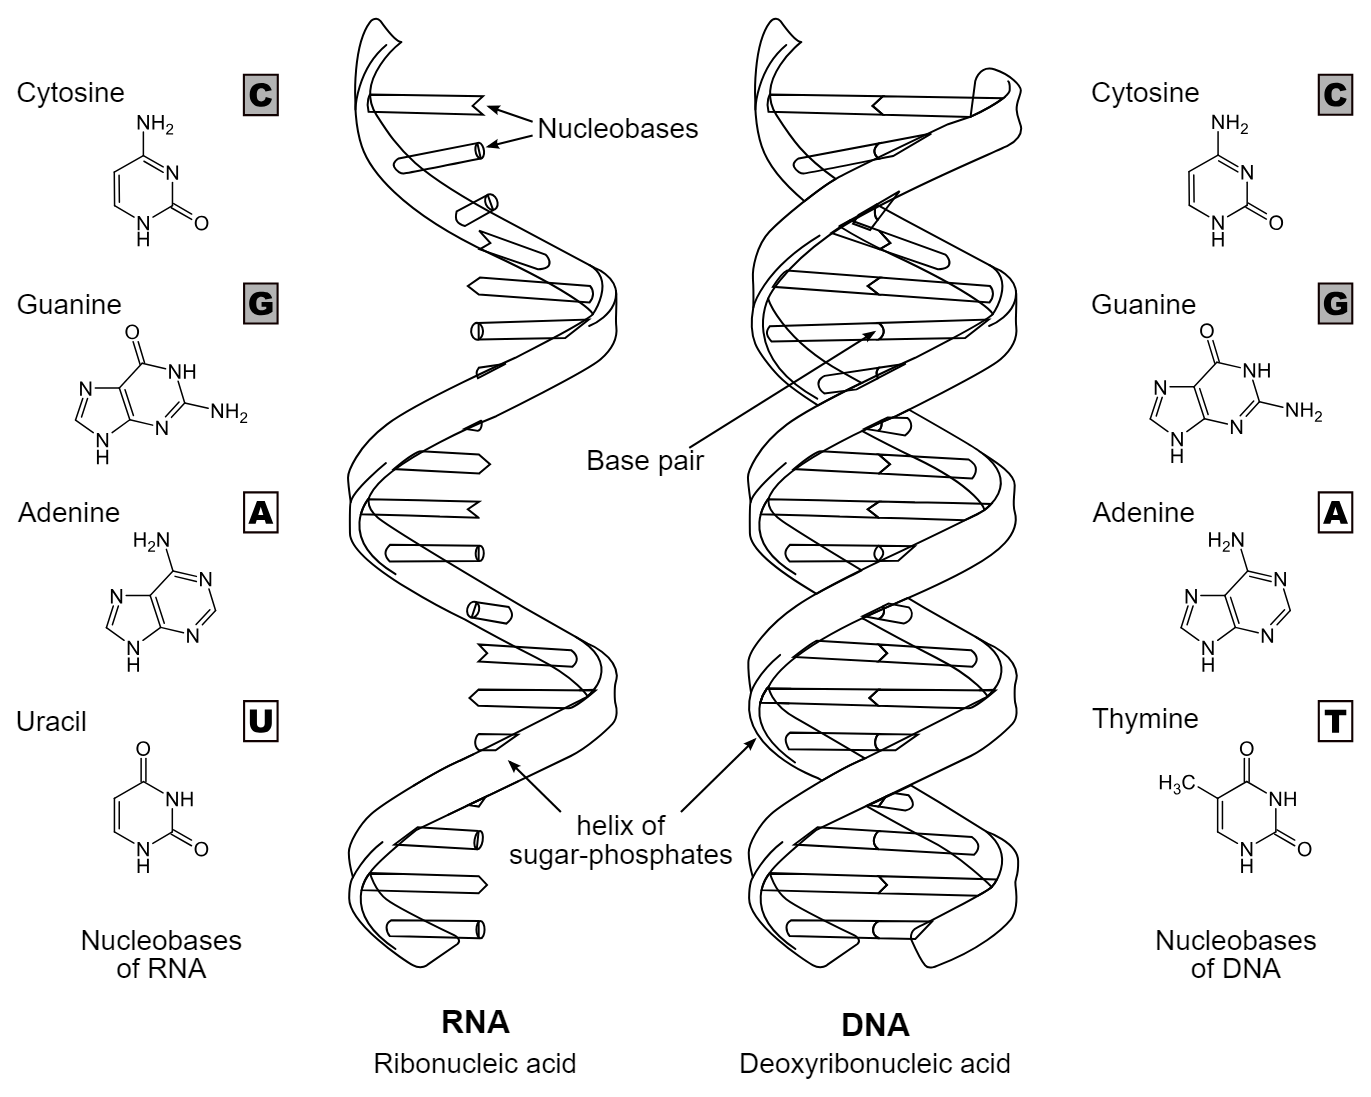
\includegraphics[width=1\textwidth]{rnadna.png}
    \end{center}
  \end{figure}
\end{frame}

\begin{frame}{What Is an Aptamer?}
\begin{itemize}
  \item Aptamers are synthetic RNA molecules that bind to a specific target
  \item Similar function to antibodies, but much smaller
  \item \textbf{Genetic code not expressed}
  \begin{figure}
    \begin{center}
      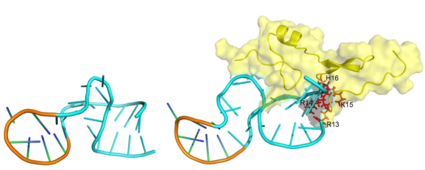
\includegraphics[width=1\textwidth]{aptamer.png}
    \end{center}  
  \end{figure}
\end{itemize}
  
\end{frame}

\begin{frame}{Comparing Aptamers}
  \begin{itemize}
    \item For TDA to work we need a notion of distance among aptamers
    \item Aptamers have two characteristics: their genetic code and their structure
    \item Distance between sequences: Levenshtein distance
    \item Distance between structures: tree distance
  \end{itemize}
\end{frame}

\begin{frame}{Distance Functions}
  \begin{itemize}
    \item The \textbf{Levenshtein distance} between two strings $a$ and $b$ is the minimum number of deletions, insertions, or substitutions needed to change $a$ into $b$.
    \begin{itemize}
      \item lev(house, mouse) = 1 (single substitution)
      \item lev(cat, tarp) = 3 (2 substitutions, 1 insertion)
      \item lev(mister, mister) = 0 (!)
    \end{itemize}
    \item The \textbf{graph edit distance} between two graphs $G$ and $H$ is the minimum number of vertex/edge insertions or deletions needed to make $G$ isomorphic to $H$.
    \begin{itemize}
      \item dist($K_n$, $K_{n-1}) = n$
      \item dist($C_n, C_k) = 2(|n-k|+1)$
    \end{itemize}
  \end{itemize}
\end{frame}

\begin{frame}{Aptamer Metrics}
  \begin{figure}
    \begin{center}
      \hspace*{-.75cm}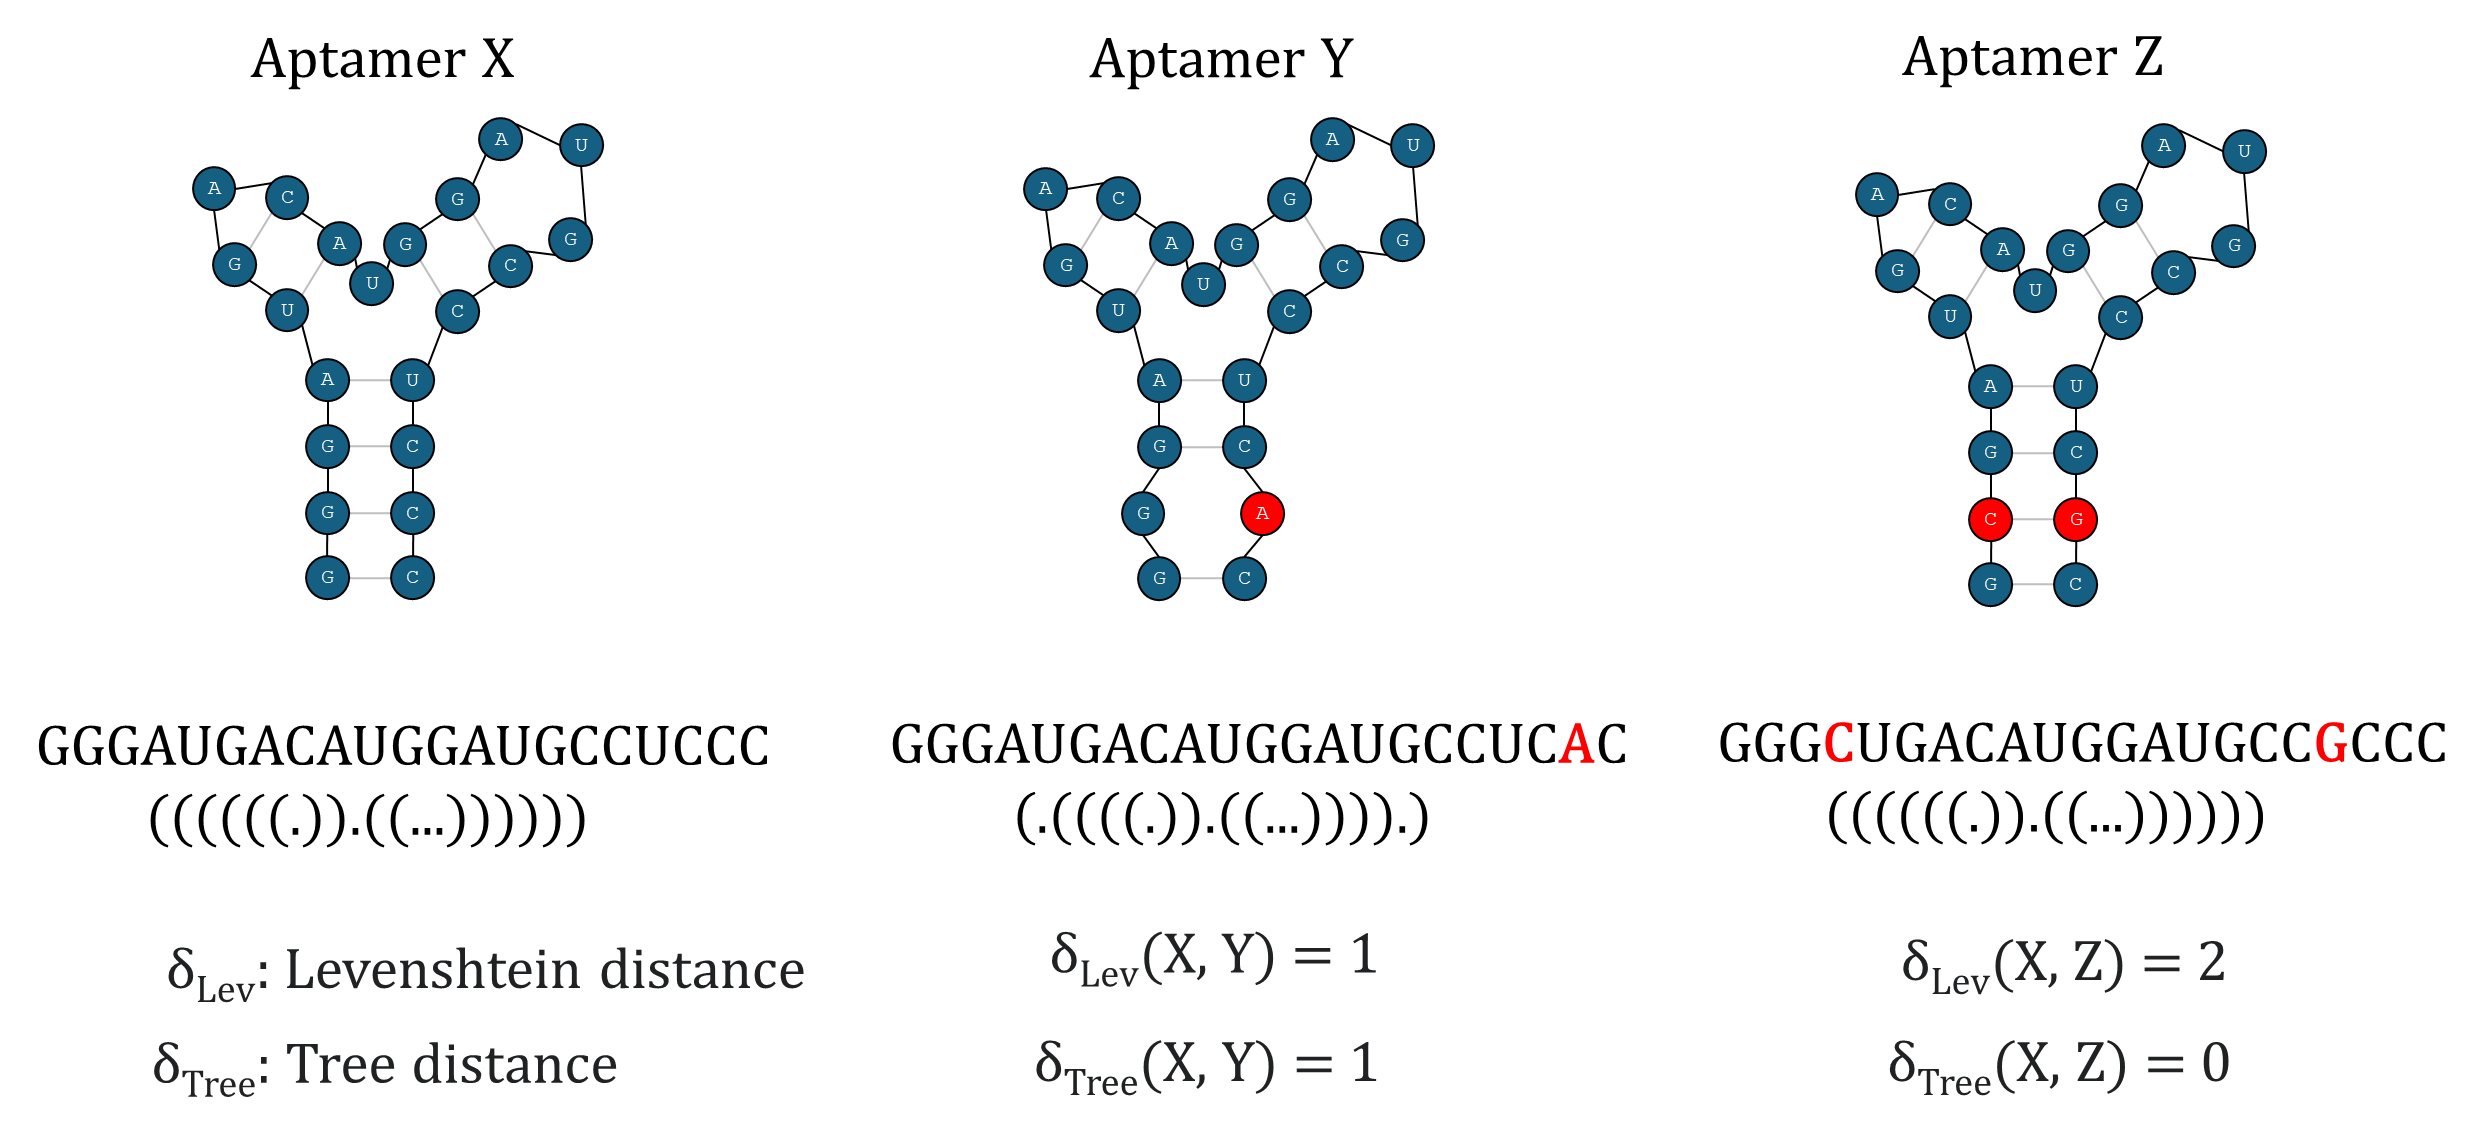
\includegraphics[width=1.15\textwidth]{aptamers.png}
    \end{center}
  \end{figure}
\end{frame}

\begin{frame}{Aptamer Clustering With Mapper}
  \begin{itemize}
    \item Flavor: Refined Ballmapper
    \item Idea: Ball using tree distance, cluster using Levenshtein distance
    \item Clustering method: single linkage hierarchical
    \item Vertices of the graph are clusters of aptamers related in both sequence and structure
    \item Graph structure may highlight families of aptamers or reveal other insights
  \end{itemize}
\end{frame}

\begin{frame}{Big Mapptamer Graph}
  \begin{figure}
    \begin{center}
      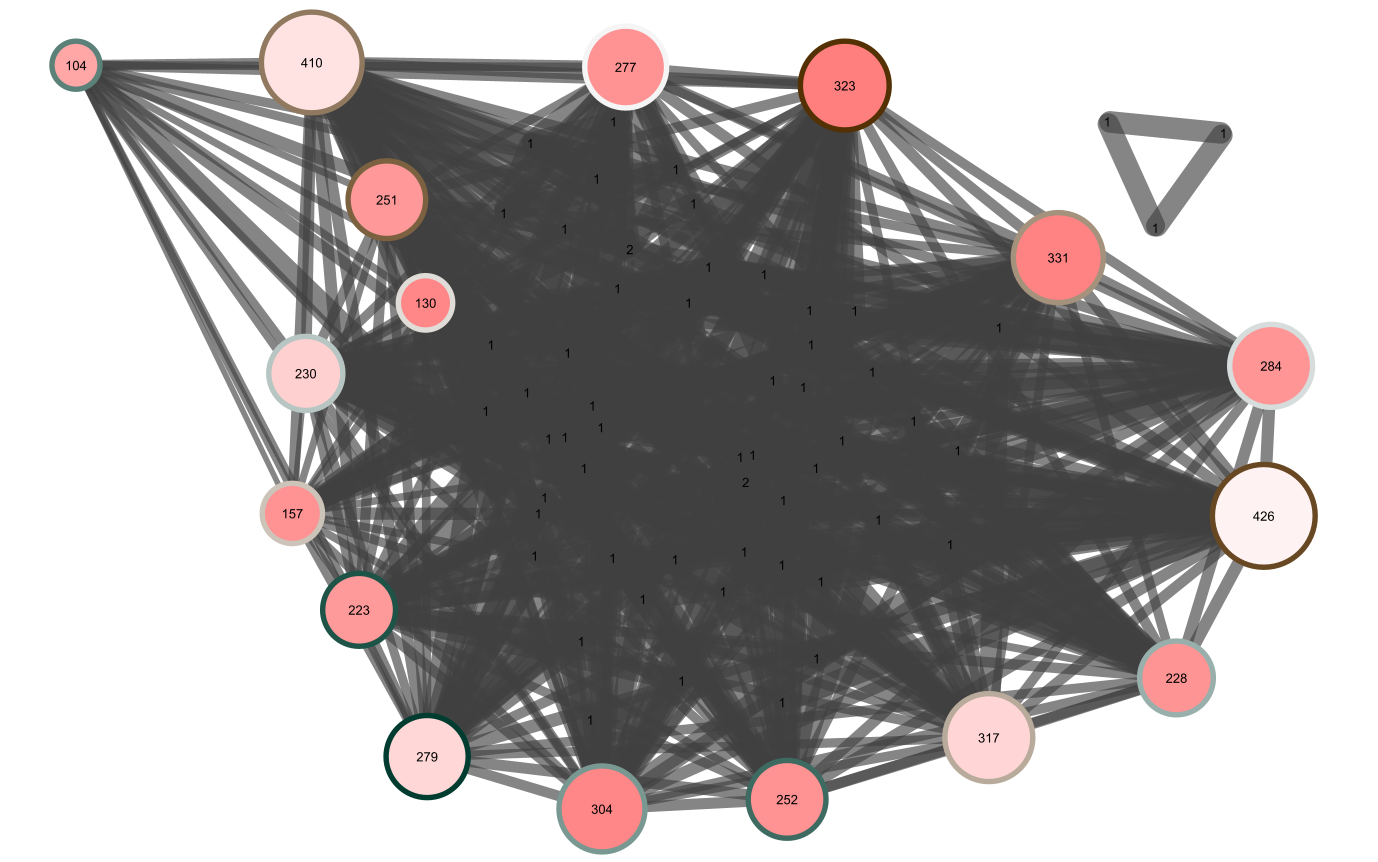
\includegraphics[width=1\textwidth]{bigmapptamer.png}
    \end{center}
  \end{figure}
\end{frame}

\begin{frame}{Pruned Mapptamer Graph}
  \begin{figure}
    \begin{center}
      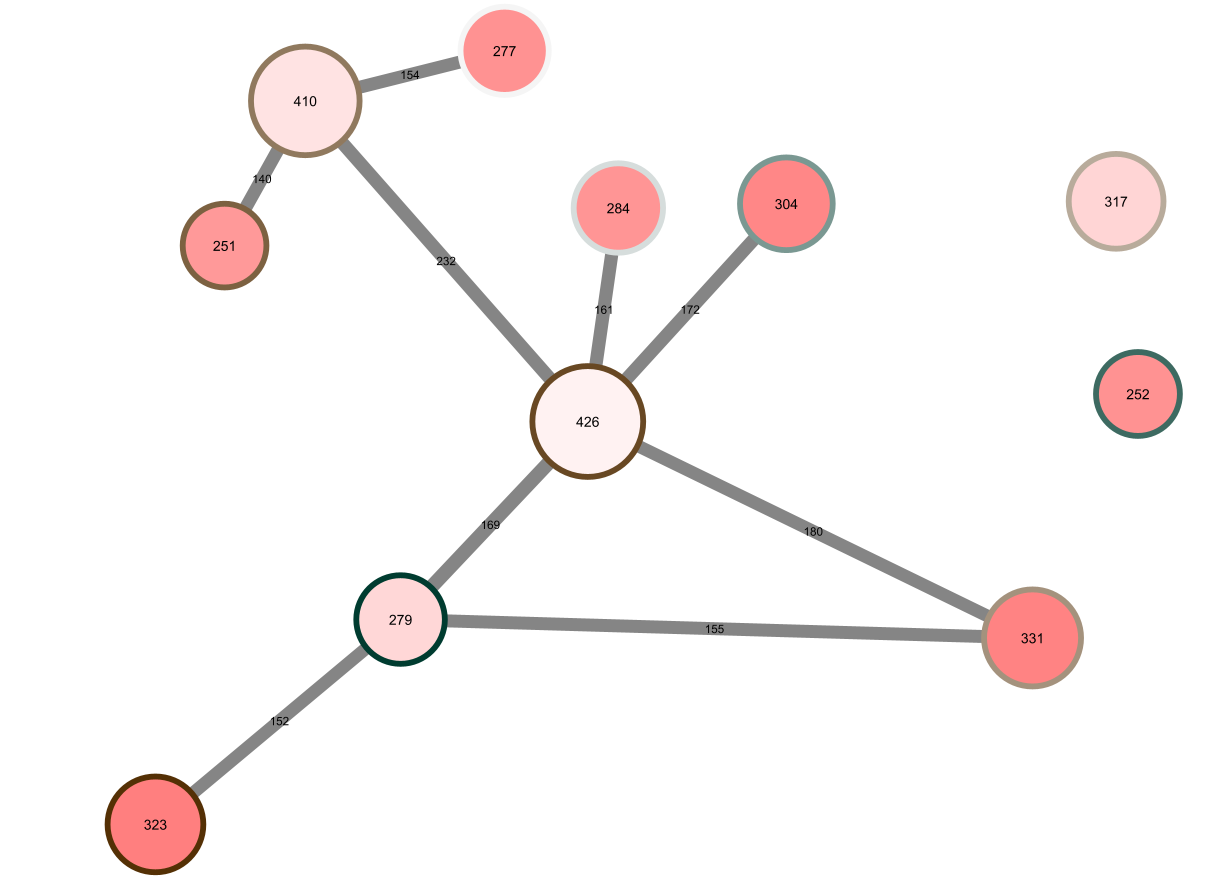
\includegraphics[width=1\textwidth]{prunedmapptamer.png}
    \end{center}
  \end{figure}
\end{frame}

\section{Mapping out Future Directions}
\begin{frame}{Other Clustering Algorithms}
  \begin{itemize}
    \item Hierarchical:
    \begin{itemize}
      \item Complete linkage: $$\ell(A, B) = \max_{a\in A, b\in B}\{d(a,b)\}$$
      \item (Unweighted) average linkage: $$\ell(A,B) = \frac{1}{|A||B|}\sum_{a\in A}\sum_{b\in B}d(a,b)$$
    \end{itemize}
    \item $k$-means
    \item Topological Mode Analysis Tool (ToMATo) \cite{tomato}

  \end{itemize}
  \begin{figure}
    \begin{center}
      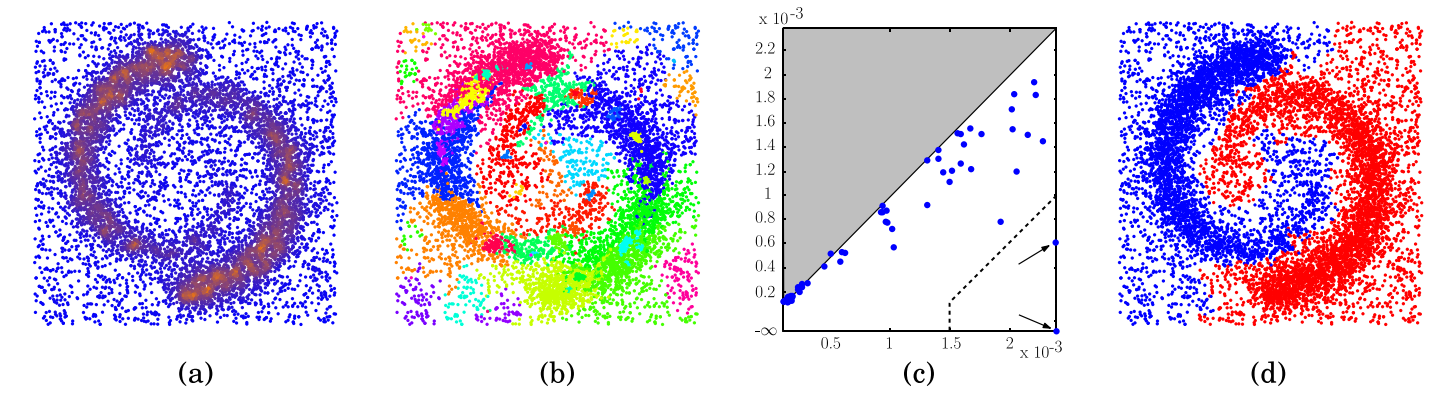
\includegraphics[width=1\textwidth]{tdaclusters.png}
    \end{center}
  \end{figure}
\end{frame}


\begin{frame}{Refined Ballmapper and Graph Theory}
  \begin{itemize}
    \item A function $\phi$ between the vertices of two graphs $G$ and $H$ is called a \textbf{graph homomorphism} if $uv\in E(G)$ implies $\phi(uv)\in E(H)$.
    \item $G$ and $H$ are called \textbf{homomorphically equivalent} (hom-equivalent) if there exist graph homomorphisms $f: G\to H$ and $g: H\to G$.
  \end{itemize}
  \begin{figure}
    \begin{center}
      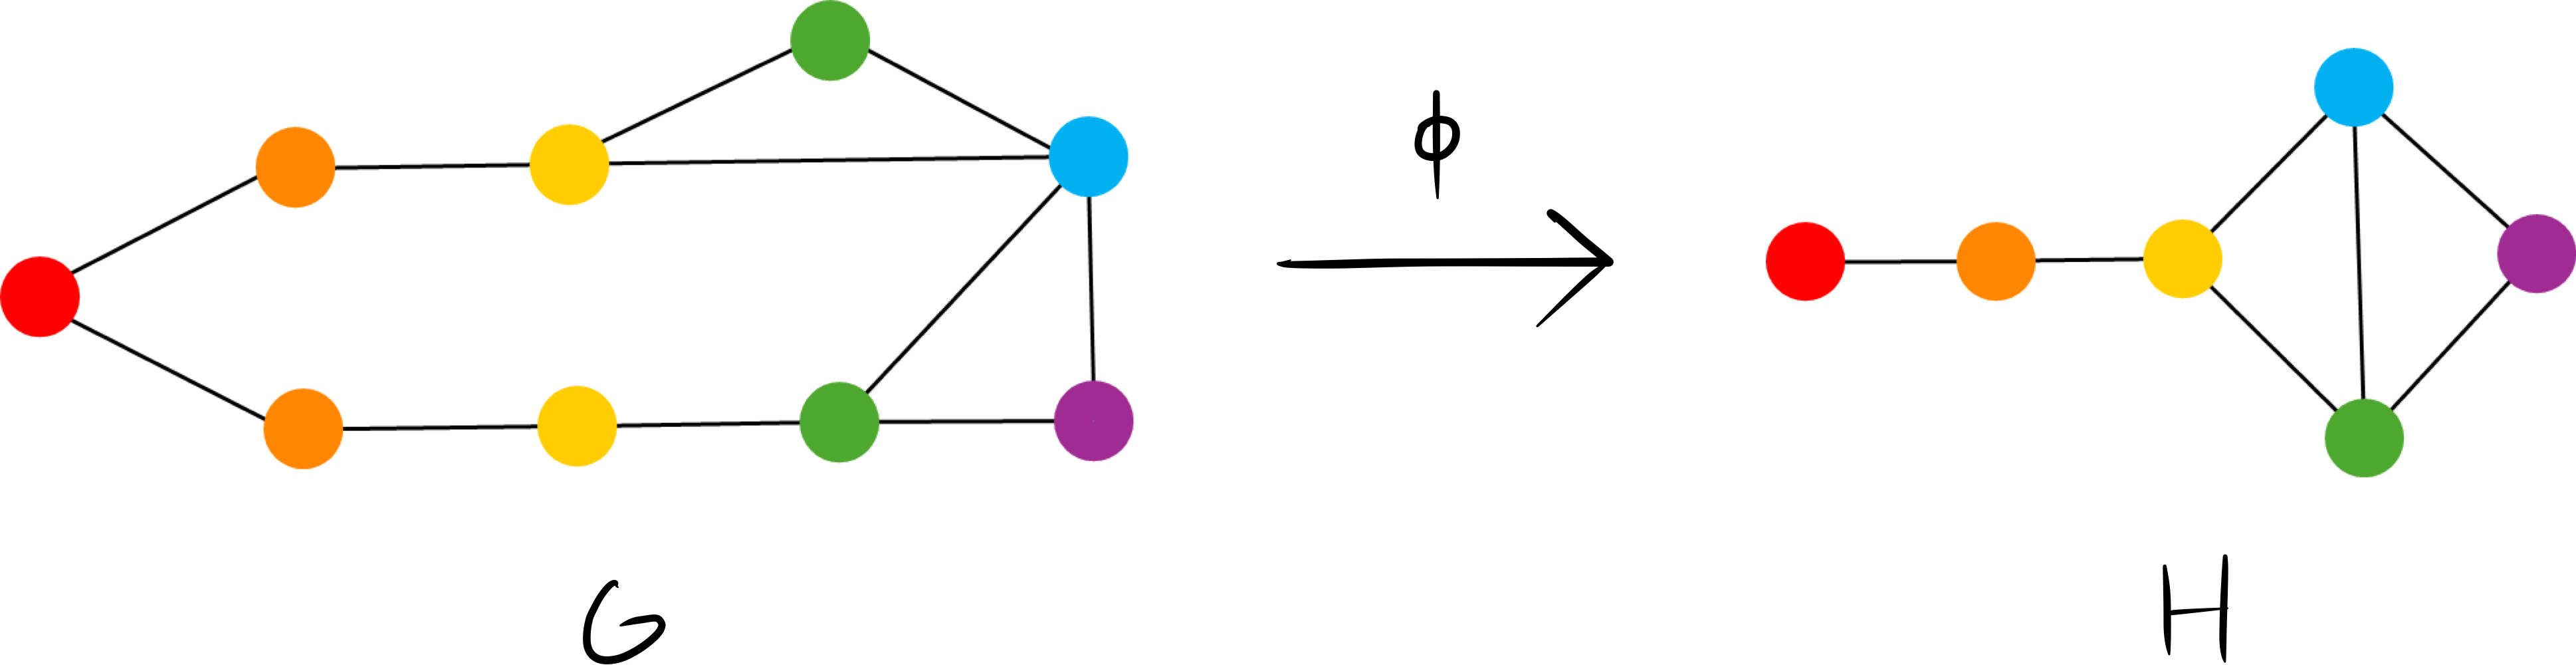
\includegraphics[width=1\textwidth]{graphhomo.png}
    \end{center}
  \end{figure}
\end{frame}

\begin{frame}{Why Might We Care? Possibility: Cores}
  \begin{itemize}
    \item A \textbf{core} $C$ of a graph $G$ is a graph such that $G$ and $C$ are hom-equivalent, and $C$ is the smallest such graph.
    \begin{itemize}
      \item Complete graphs, odd cycles, etc
    \end{itemize}
    \item Every finite graph has a core, and it is unique (up to isomorphism).
    \item Graphs with the same cores are necessarily hom-equivalent, and vice versa.
    \item Core-finding complexity: NP-complete :(
    \item Applications to relational algebra
  \end{itemize}
\end{frame}

\begin{frame}{Example Equivalence via Core}
  \begin{figure}
    \begin{center}\hspace*{-.3cm}
      \only<1>{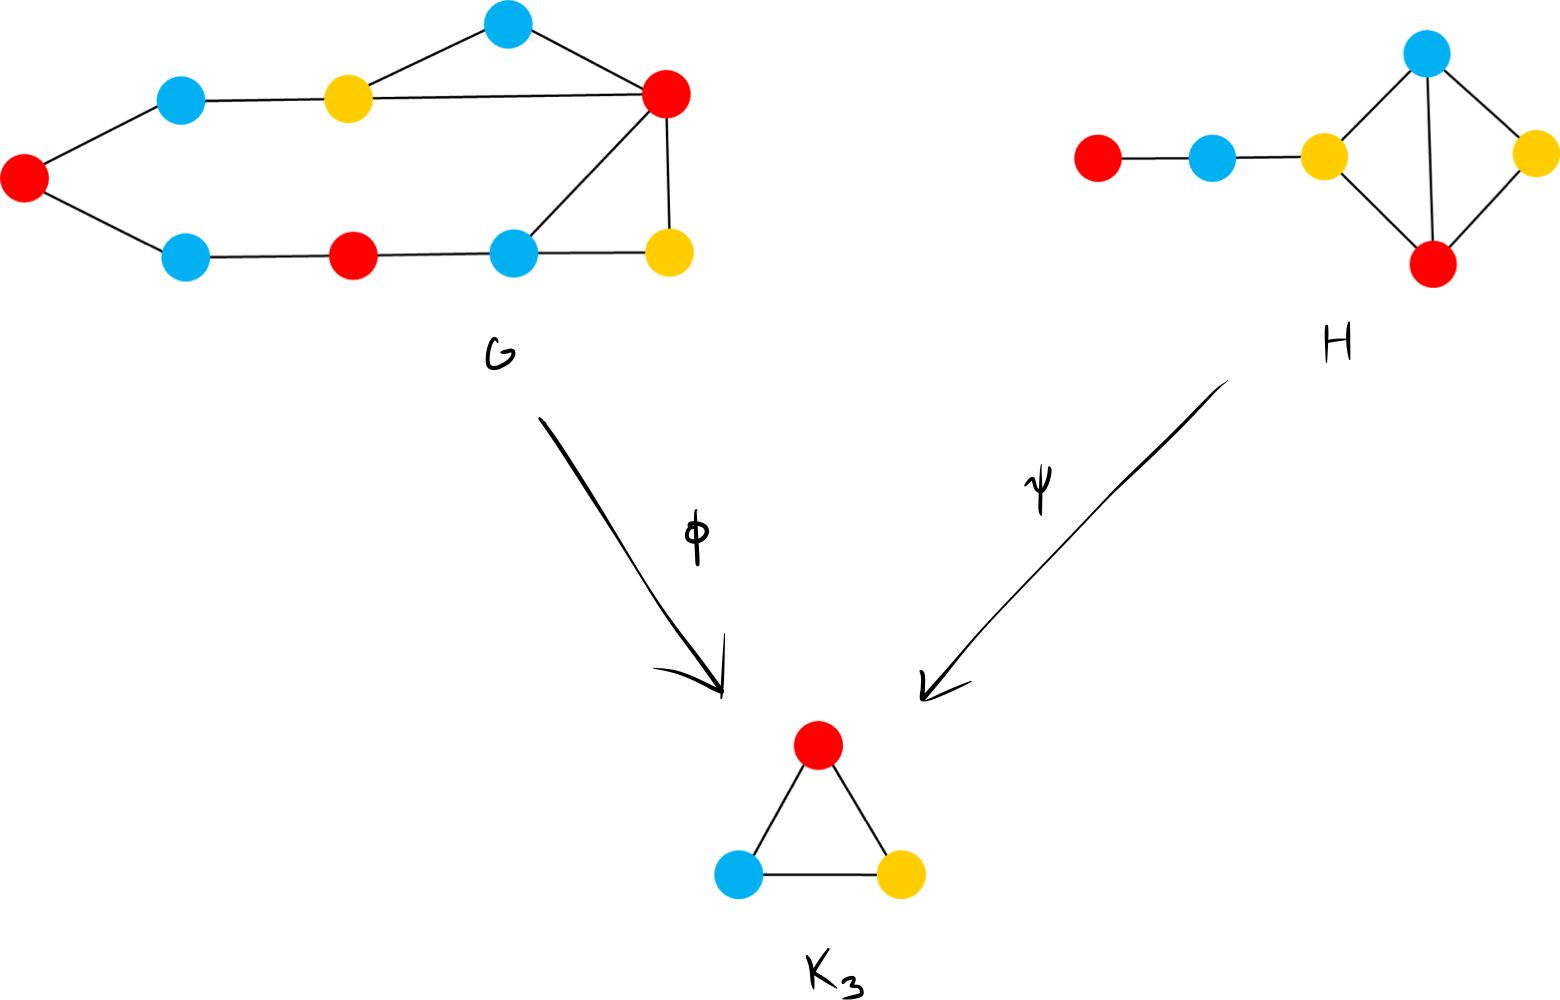
\includegraphics[width=1.05\textwidth]{graphcore.png}}
      \only<2>{\includegraphics[width=1.05\textwidth]{graphcoreinclusion.png}}
    \end{center}
  \end{figure}
  \begin{figure}
    \begin{center}\vspace*{-1.65cm}\hspace*{-.3cm}
      \only<3>{\includegraphics[width=1.05\textwidth]{graphcorefull.png}}
    \end{center}
  \end{figure}
\end{frame}

\begin{frame}{Stability}
  
\end{frame}

\begin{frame}{Persistence}
  
\end{frame}

\begin{frame}{Return of Reeb}
  
\end{frame}

\subsection{Biology}
\begin{frame}{More Aptamers}
  
\end{frame}

\begin{frame}{Neuroscience}

\end{frame}

\begin{frame}
  \printbibliography
\end{frame}

\end{document}